\documentclass[9pt]{article}
\usepackage[letterpaper, margin=2cm]{geometry}
\usepackage[utf8]{inputenc}
\usepackage[sfdefault]{inter}
\usepackage[T1]{fontenc}
\usepackage{amsmath}
\usepackage{graphicx, caption}
\usepackage{xcolor}
\usepackage{subcaption}
\usepackage{siunitx}
\usepackage{subfig}
\usepackage{booktabs}
\usepackage{tabularx}
\usepackage{multirow}
\usepackage{pdflscape}
\usepackage{mhchem}
\let\temp\rmdefault
\usepackage{fourier}
\let\rmdefault\temp

\usepackage[
  backend=biber,
  style=ieee
]{biblatex}
\addbibresource{spacecraft.bib}

% Title Page
\title{\Huge SARGE\\\Large Final Report}
\author{Jimmy Vaughan\\(101 156 687)}


\begin{document}
\begin{figure}[t]
  \centering
  
\includegraphics[width=.7\linewidth]{CarletonLogo}
\end{figure}
\maketitle
\pagenumbering{gobble}
\clearpage
\tableofcontents
\clearpage
\pagenumbering{arabic}
\section{Introduction}
SARGE, \textbf{S}ynthetic~\textbf{A}perture~\textbf{R}adar:~\textbf{G}reenhouse~\textbf{E}missions, is a satellite platform designed to monitor for potential leaks of cross-Canada pipelines using synthetic aperture radar.
This report details a prelimnary design that should provide a solid starting point for further analysis and refinement.
Assumptions and estimations are necessary at this stage of development, and their presence is clearly noted in the following sections on analysis.

Preliminary design drawings are avaiable in the last appendix, Appendix~\ref{app:julia}.

\subsection{Primary Mission Objectives}
  The primary mission objective of SARGE is to monitor the entirety of Canada for the presence of greenhouse gasses that would indicate leaks in the transcontinental petrochemical pipelines.
  To this end, SARGE covers all of contiguous Canada, but does not directly cover the many islands in the far north of the territories.
  This should be acceptable, since there are no pipelines in those areas, and there is really only one pipeline above Hudson's Bay, ending just north of Mackenzie Bay, past Inuvik,~N.W.T.~\cite{pipelines}.
\subsection{Secondary Mission Objectives}
  Since SARGE covers the entirety of Canada (and Alaska, U.S.) any application of regular monitoring could be co-located on the satellite.
  Wildfire monitoring/detection, all industrial greenhouse gas emissions, and even meteorology.
  One of the only terrestrial applications SARGE is unsuited for is communications, as it is out of sight for about 2/3 of each day.

\section{Orbit Selection}
The assigned mission requirements state that this satellite is to image the entirety of Canada at least once every 14~days.
To satisfy this requirement, a geosynchronous orbit with a nonstandard high inclination (\ang{121}) was chosen.
The ground track of a conical SAR (shown in Figure~\ref{fig:groundtrack}) with a minimum elevation angle of \ang{75} covers the entirety of contiguous Canada.

\begin{figure}[hb]
  \centering
  \captionsetup{width=.75\linewidth,font={small},labelfont={bf}}
  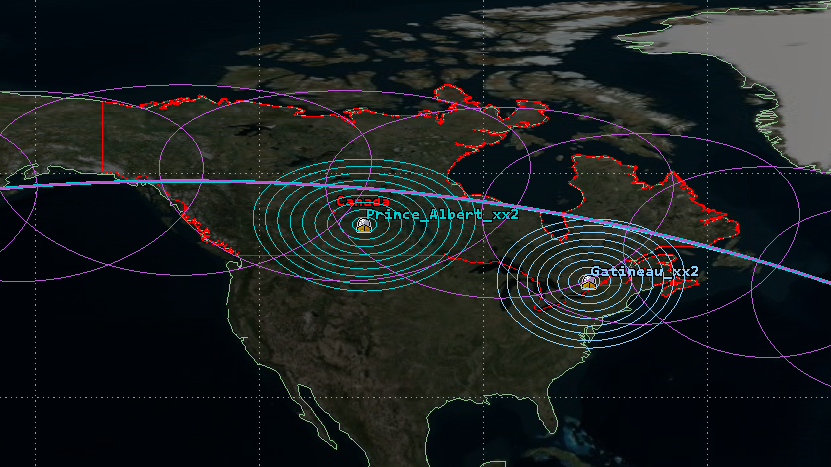
\includegraphics[width=12cm]{groundtrack}
  \caption{Ground swath of SARGE over continental Canada. Ground stations are shown in teal and sky blue, and the majority of Canada is outlined in red ($A\approx\qty{8.342e6}{\square\kilo\metre}$). The magenta circles show the coverage of the SAR beam at some discrete points in time.}
  \label{fig:groundtrack}
\end{figure}

The orbital parameters are summarized in Table~\ref{tab:orbit}.
We can see that the chosen orbit is a circular retrograde orbit with a period of about one sidereal day.
This regularity allows the satellite to image, process, and transmit one~fourteenth of Canada each day, with a consistent and regular ground station access window.

\begin{table}[h]
  \centering
  \captionsetup{width=.75\linewidth,font={small},labelfont={bf}}
    \begin{tabular}{r S|r S}
      \toprule
      \multicolumn{4}{c}{Basic Orbital Parameters}\\
      \midrule
      Period $P$ & \qty{86170.5}{\second} & Arg. of Perigee $\omega$ & \ang{0} \\
      Eccentricity $\epsilon$ & \num{0.0} & LAN $\Omega$ & \ang{50} \\
      Inclinination $i$ & \ang{121} & True Anomaly $\nu$ & \ang{30} \\
      \midrule %\midrule
      \multicolumn{4}{c}{Derived Quantities}\\
      \midrule
      Orbit Radius $r$ & \qty{42166.26}{\kilo\metre} & Orbital Altitude $h$ & \qty{35788.12}{\kilo\metre} \\
      Velocity $v$ & \qty{3.074}{\kilo\metre\per\second} & Orbits per Day $n$ & \qty{1.002663}{\per\day} \\
      \bottomrule
    \end{tabular}
    \caption{Orbital parameters and convenient derived quantities.}
    \label{tab:orbit}
\end{table}

At high altitudes, like GEO, the gravitational forces of the Sun and the Moon become significant, but air drag is generally negligible~\cite[p. 81]{sse}.
As well, the high inclination of SARGE allows it to avoid most of the clutter in the GEO belt, since most of the objects are within <\ang{5} inclination~\cite[p. 140]{sme}.
Another advantage is the lack of an eclipse time in service (there may be a short eclipse during transit to orbit), as shown in Figure~\ref{fig:eclipse} in Section~\ref{sys:power}.
Stationkeeping requirements are also quite low, as explored in Appendix~\ref{app:stnkeep} and mentioned in Section~\ref{sys:prop}, since the oblateness of Earth is primarily a factor in lower inclination orbits.

\section{Spacecraft Bus}
\subsection{Mass and Power Budget}
According to David Everett of the NASA Goddard Space Flight Center, the first of the three steps of mass estimation is ``A rough order of magnitude based on payload mass''~\cite[p. 399]{sme}.
Given that sentiment, and approximate sizing of the power array (see Section~\ref{sys:power}), the initial mass estimate is based on data representative of mission type \textit{and} historical data given in Table~14-18, which can be found in Appendix~\ref{app:refs}, Figure~\ref{fig:1418}, and summarized in Table~\ref{tab:mass}, with comments noted in the third column.

\begin{table}[h]
  \centering
  \captionsetup{width=.75\linewidth,font={small},labelfont={bf}}
  %\begin{tabularx}{.8\linewidth}{l|r r X}
  \begin{tabular}{l|r r l}
    \toprule
    Subsystem & Mass\% & Mass & Comments \\
    \midrule
    Payload & \qty{32}{\percent} & \qty{200}{\kilo\gram} & Provided in requirements \\
    Structure \& Mechanisms & \qty{24}{\percent} & \qty{150}{\kilo\gram} & Taken from Table~14-18\\
    Thermal Control & \qty{6}{\percent} & \qty{36.}{\kilo\gram} & \qty{11}{\kilo\gram} taken from Power subsystem\\ 
    Power (incl. harness) & \qty{13}{\percent} & \qty{82}{\kilo\gram}&Less than usual since no eclipse\\
    TT\&C & \qty{4}{\percent} & \qty{25}{\kilo\gram}&Taken from Table~14-18\\
    Data Processing & \qty{3}{\percent} & \qty{19}{\kilo\gram}&''\\
    ADCS & \qty{8}{\percent} & \qty{50}{\kilo\gram}& \qty{13}{\kilo\gram} taken from Power\\
    Propulsion & \qty{7}{\percent} & \qty{44}{\kilo\gram}&Taken from Table~14-18\\
    Other & \qty{3}{\percent} & \qty{19}{\kilo\gram}&''\\
    \midrule 
    Total Dry Mass & \qty{100}{\percent} & \qty{625}{\kilo\gram} & \\
    Propellant & \qty{142}{\percent} & \qty{885}{\kilo\gram} & Double expected amount in Table~14-18\\
    Kick motor & \qty{12}{\percent} & \qty{75}{\kilo\gram} & Estimated mass of a jettisonable liquid motor\\
    \midrule 
    Wet Mass & & \qty{1585}{\kilo\gram} & \\
    \bottomrule
  \end{tabular}
  \caption{Preliminary mass budget estimation, based on provided payload mass and the listing for ``High Earth'' in the SME-SMAD~\cite{sme}.}
  \label{tab:mass}
\end{table}

The breakdown of the power subsystem is available in Table~\ref{tab:powerbreakdown} in Section~\ref{sys:power}.
Historical basis for the amount of propellant needed was insufficient for this particular satellite, primarily because of the steep inclination and the high-$\Delta V$ maneuvers required, detailed in Section~\ref{sys:prop}.
The total wet mass still comes in at far less than the SpaceX Falcon~9's maximum lift-off mass of \qty{5800}{\kilo\gram} (Table~\ref{tab:launchertrade}), so a shared launch is still feasible (especially given the compact nature of SARGE).


  Like the Mass Budget in Table~\ref{tab:mass}, the preliminary power budget below in Table~\ref{tab:power} is based on David~Everett's chapter of the SME-SMAD, Table~14-20 (Appendix~\ref{app:refs}, Figure~\ref{fig:1420}).
  This time, however, a modification to the suggested weights in Table~14-20 was made to accomodate the two one-axis solar array gimbals notes in Section~\ref{sec:configuration}. 
The payload power proportion was thus lessened by \qty{2}{\percent}, from \qty{35}{\percent} to \qty{33}{\percent} to give a corresponding power proportion of \qty{2}{\percent} to the Structures~\&~Mechanisms subsystem.
The solar array and battery sizing calculations are presented in Section~\ref{sys:power}.

\begin{table}[h]
  \centering
  \captionsetup{width=.75\linewidth,font={small},labelfont={bf}}
  \begin{tabular}{l|r r l}
    \toprule
    Subsystem & Power\% & Avg. Power & Comments \\
    \midrule
    Payload & \qty{33}{\percent} & \qty{350}{\watt} & Specified in requirements, mod. from Table~14-20 \\ 
    Structure \& Mechanisms & \qty{2}{\percent} & \qty{21}{\watt} & Mod. from Table~14-20 \\
    Thermal & \qty{14}{\percent} & \qty{148}{\watt} & Taken from Table~14-20 \\
    Power (incl. harness) & \qty{7}{\percent} & \qty{75}{\watt} & ''\\
    TT\&C & \qty{16}{\percent} & \qty{170}{\watt} & ''\\
    Data Processing & \qty{10}{\percent} & \qty{106}{\watt} &''\\
    ADCS & \qty{16}{\percent} & \qty{170}{\watt}&''\\
    Propulstion & \qty{2}{\percent} & \qty{21}{\watt} & ''\\
    \midrule
    Total & \qty{100}{\percent} & \qty{1061}{\watt} &\\
    \bottomrule
  \end{tabular}
  \caption{Preliminary power budget estimation, based on provided payload mass and the listing for ``High Earth'' in the SME-SMAD~\cite{sme}, modified to allow for powered mechanisms.}
  \label{tab:power}
\end{table}

\subsection{Configuration}\label{sec:configuration}
The configuration of SARGE is a nadir-pointing 3-axis stabilized solar-powered satellite.
The two solar arrays are gimbaled in one axis with a range of $\pm\ang{10}$ to account for the slight variation in the spacecraft's orientation with respect to the sun as it travels along its orbital path (this angle was found in Appendix~\ref{app:orbplanes}).
The size of the spacecraft can be estimated using the relations listed in Slideshow~3, Configuration, and shown in Table~\ref{tab:sizeest} below.

\begin{table}[h]
  \centering
  \captionsetup{width=.75\linewidth,font=small,labelfont=bf}
  \begin{tabular}{lll}
    \toprule
    Characteristic & Equation & Estimate \\
    \midrule
    Volume (\si{\meter\cubed}) & $V=0.01M$ & \qty{15.85}{\meter\cubed}\\
    Linear Dimension (\si{\meter}) & $L=0.25M^{1/3}$ & \qty{2.91}{\meter}\\
    Body Area (\si{\meter\squared}) & $A_b=V/L$ & \qty{5.44}{\meter\squared}\\
    Moment of Inertia (\si{\kilo\gram\meter\squared}) & $I=0.01M^{5/3}$ & \qty{2155}{\kilo\gram\meter\squared}\\
    \bottomrule
  \end{tabular}
  \caption{Estimate of spacecraft dimensions, where $M$ is spacecraft wet mass in \si{\kilo\gram}.}\label{tab:sizeest}
\end{table}

(Comment on the estimations). The mark is actually for assumptions for calculations? Idk, I modelled the satellite to fit the payload bruh.


An annotated isometric view of the preliminary design/layout is shown in Figure~\ref{fig:iso}.

\begin{figure}[h]
  \centering
  \captionsetup{width=.75\linewidth,font=small,labelfont=bf}
  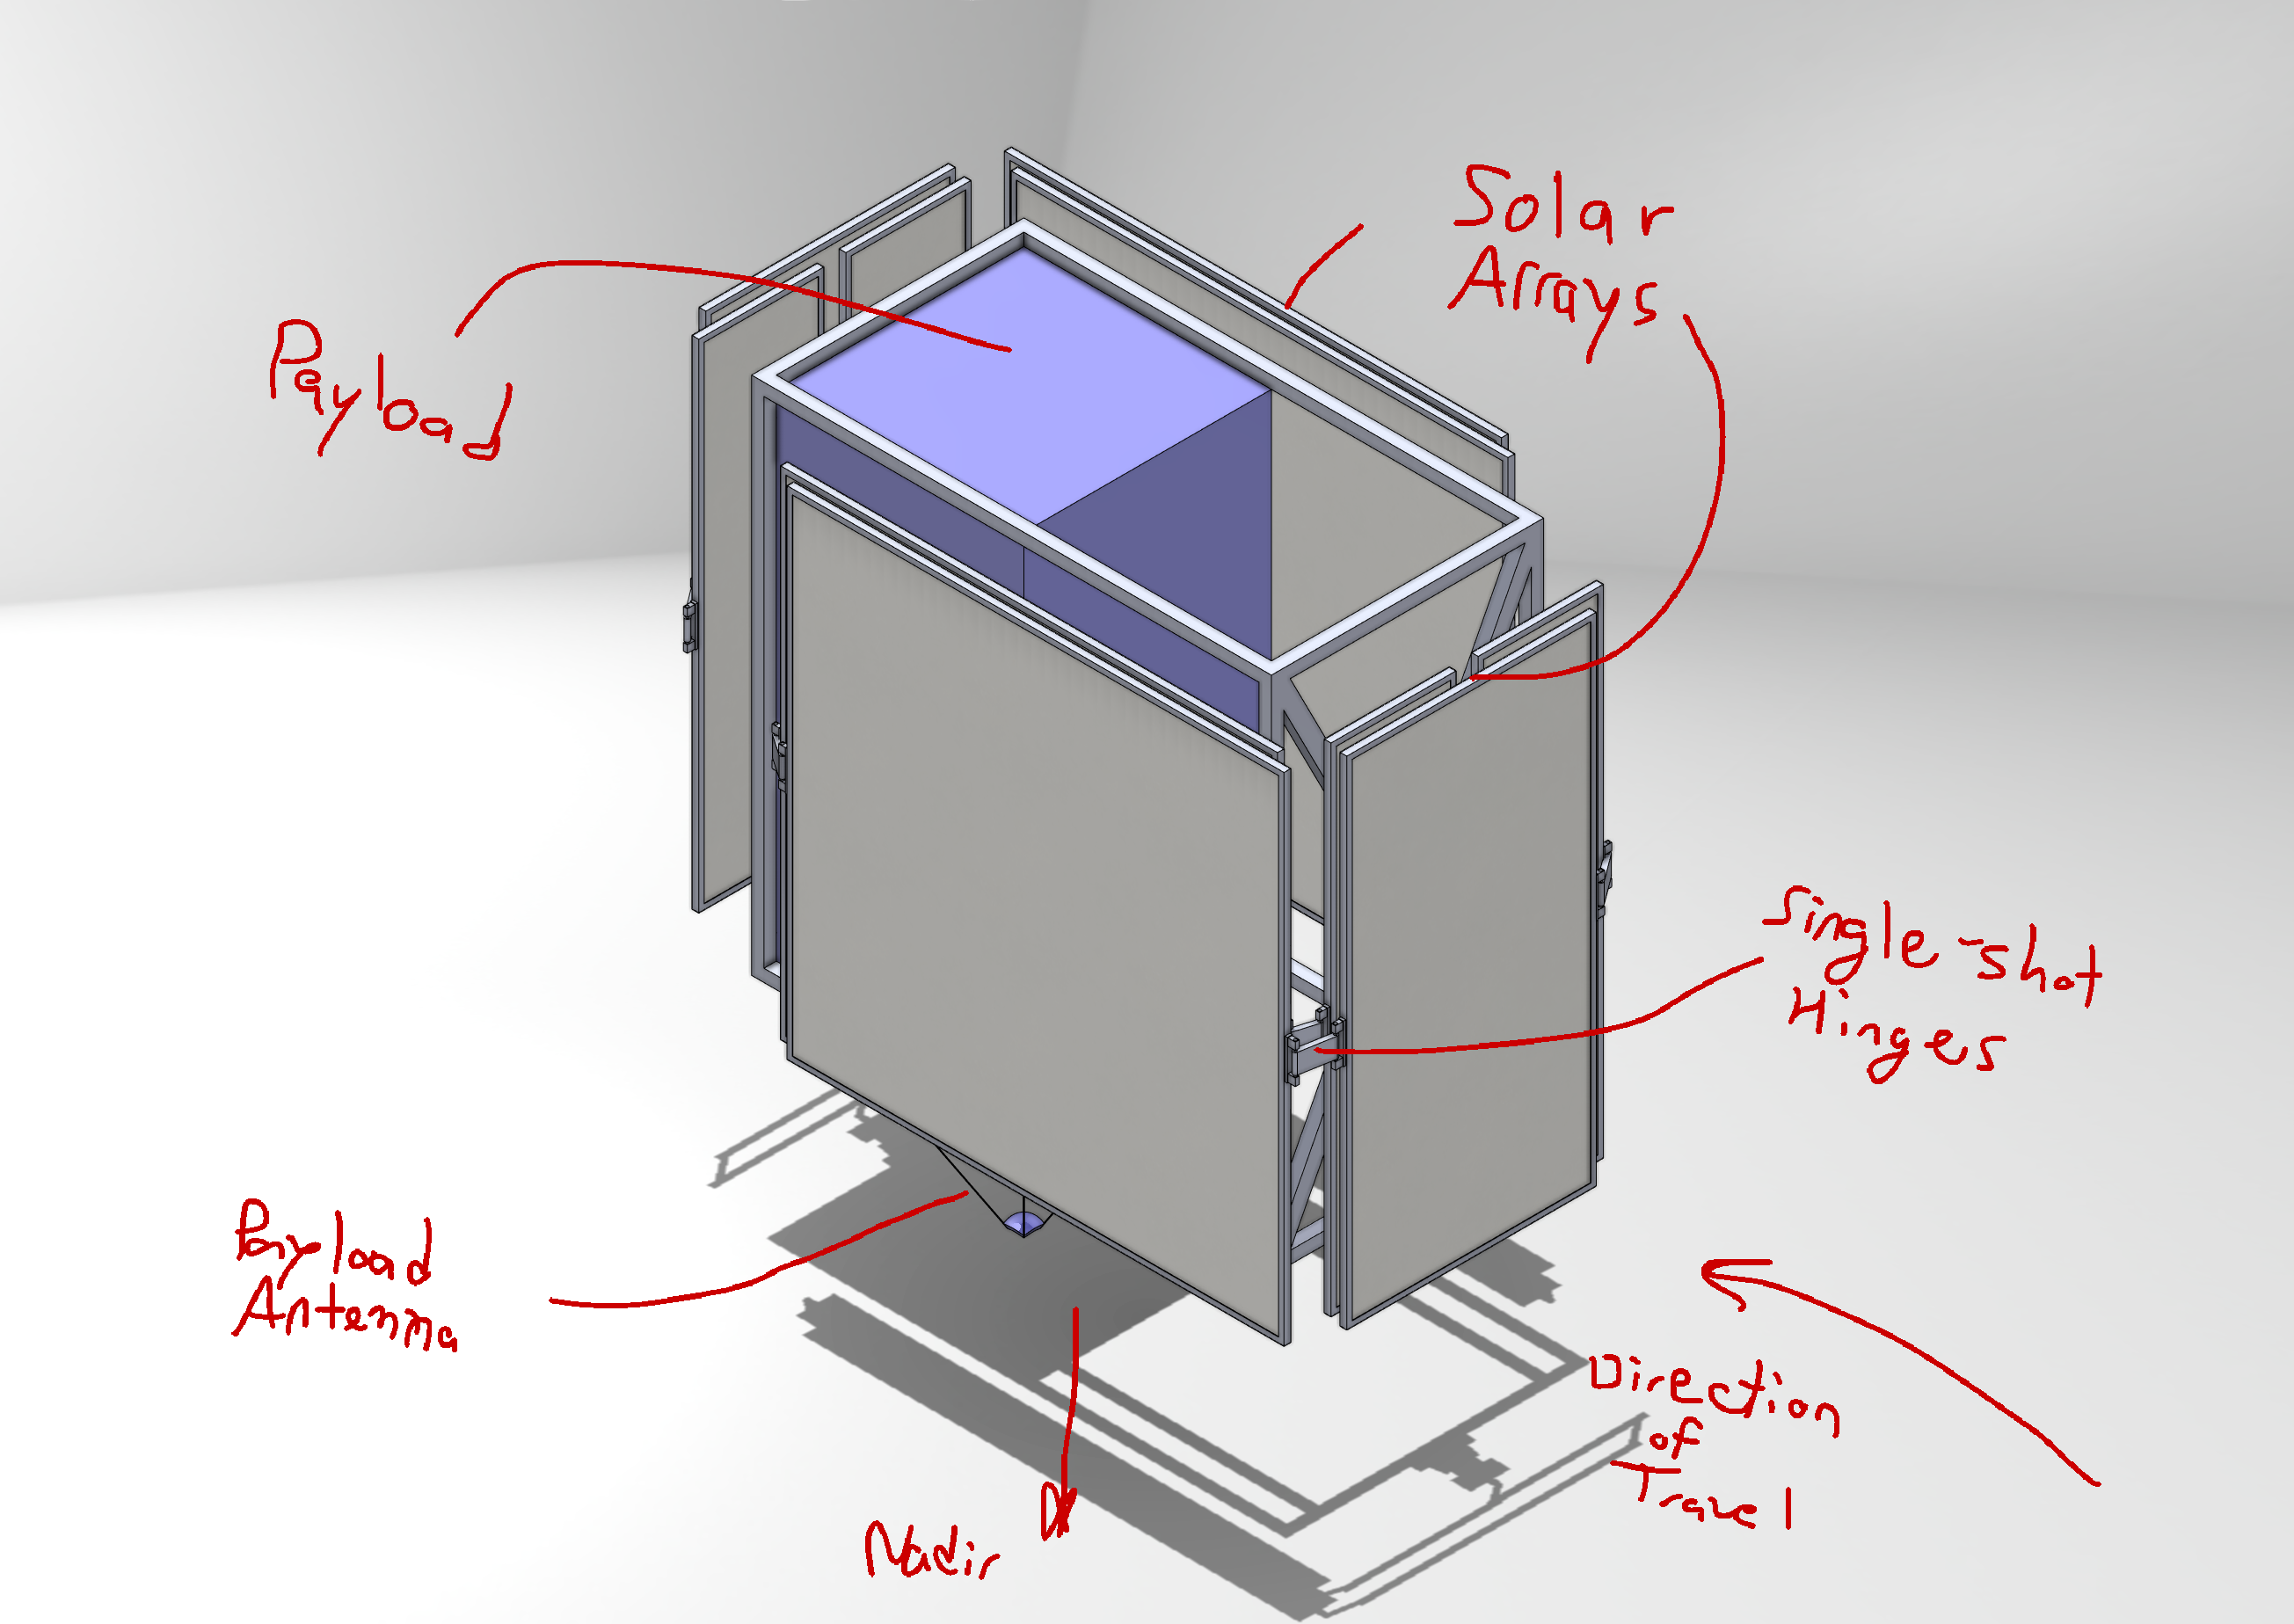
\includegraphics[width=.4\linewidth]{iso}
  \caption{Isometric view of the satellite with annotation in red to aid understanding.}
  \label{fig:iso}
\end{figure}

As can hopefully be seen, the major components currently include 2 solar arrays, articulated only for launching, via single-shot hinges at each meeting point.
These arrays are gimbaled in one axis, shown in the front view, Figure~\ref{fig:front}.
The direction of travel is shown in Figure~\ref{fig:iso}, as well as the nadir pointing direction.

\begin{figure}[h]
  \centering
  \captionsetup{width=.75\linewidth,font=small,labelfont=bf}
  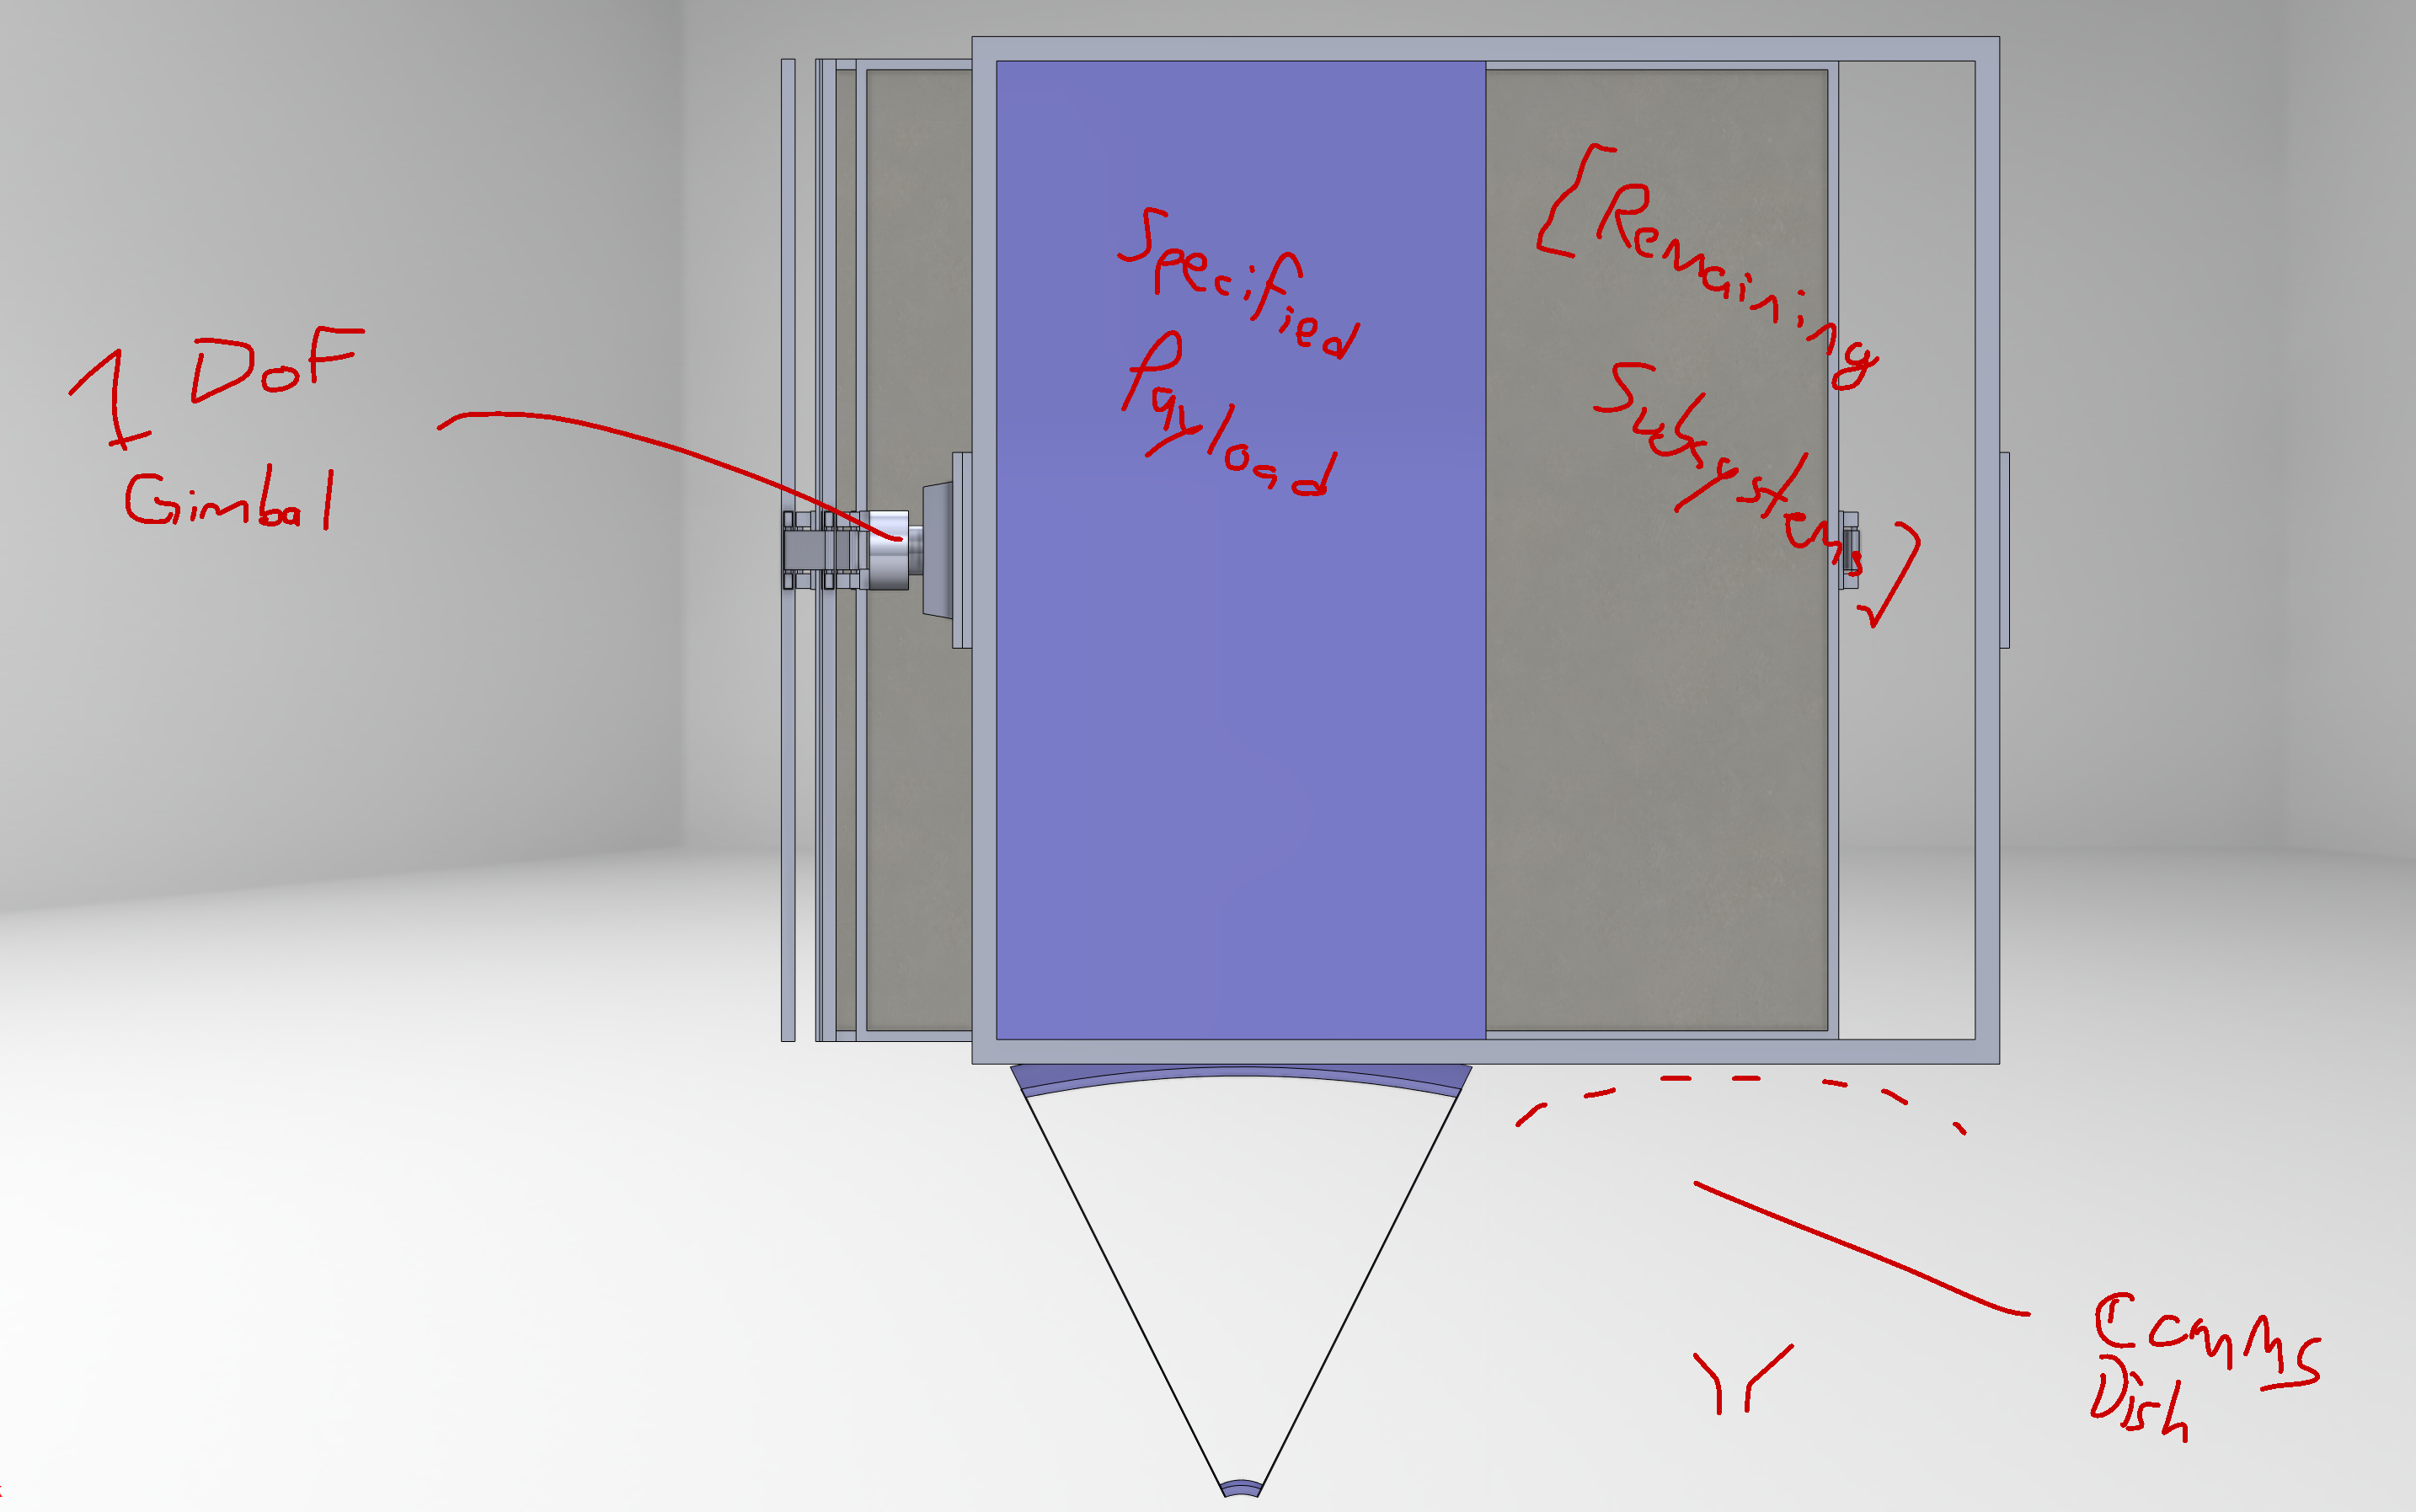
\includegraphics[width=.4\linewidth]{front}
  \caption{Front view of SARGE with annotation in red. One of the solar panel arrays is hidden so as not to obstruct the interior of the frame.}
  \label{fig:front}
\end{figure}

Since the masses of the solar arrays are identical, and they are symmetric about the nadir axis, and since the mass proportion of the payload is only around \qty{32}{\percent} of the total dry mass, the remaining subsystems should make it so that the center of mass is not located within the payload container.
This means that an ADCS system with reaction wheels should be able to be located directly in line with all three axes relative to the center of inertia, so pointing should be easily controllable.
The remaining subsystems will all ideally fit in the remaining payload-sized area to the right of the payload in Figure~\ref{fig:front}.

More engineering drawings are available in Appendix~\ref{app:julia}.



Drawings (3.5)

Justification (2)


\subsection{Preliminary Design of Spacecraft Subsystems}
\subsubsection{Communications Subsystem}\label{sys:comms}
Based on both slide deck 6, ``TTC'', and select portions of the SME-SMAD, the uplink and downlink link budgets are summarized in Table~\ref{tab:link}.
As well, the downlink and uplink frequencies were chosen according to Professor~Jim~Wight's course handout for ELEC~4509.
It's noted in that handout that frequency ranges 7.25-7.30~GHz and 7.975-8.025~GHz are reserved for downlink and uplink satellite communications, respectively~\cite[II, p. 3]{commlinks}.
The downlink budget was conceived using the data rate/budget calculations in Appendix~\ref{app:linkbudget}.
As a quick summary, the amount of data transmitted per 14 days is about \qty{1}{\tera\byte}, with a daily access window of \qty{9.5}{\hour} and a downlink data rate during that window of about \qty{2.5}{\mega\byte\per\second}, for a (QPSK-encoded) bandwidth of about \qty{12}{\mega\hertz} on a \qty{7.275}{\giga\hertz} carrier.
\begin{table}[h]
  \centering
  \captionsetup{width=.75\linewidth,font=small,labelfont=bf}
  \begin{tabular}{c|rl|l}
    \toprule
    Uplink & Value & Unit & Comments \\
    \midrule
    $P_t$ & \num{23.01} & \si{\decibel\watt} & \qty{200}{\watt} ground transmitter assumed\\
    $G_t$ & \num{57.74} & \si{\decibel} & Eq.~\ref{eq:200}\\
    $L_\text{path}$ & \num{202.68} & \si{\decibel} & Eq.~\ref{eq:203}\\
    $L_\text{point}$ & \num{18.42} & \si{\decibel} & Eq.~\ref{eq:303}\\
    $L_\text{atmosphere}$ & \num{10.00} & \si{\decibel} & Assumed\\
    $k$ & \num{-228.60} & \si{\decibel\joule\per\kelvin} & \\
    $B$ & \num{37.00} & \si{\decibel\hertz} & Eq.~\ref{eq:201}\\
    $G_r$ & \num{6.49} & \si{\decibel} & Figure~\ref{fig:hfss}\\
    $T$ & \num{14.31} & \si{\decibel\kelvin} & Assumed\\
    \midrule
    ${C/N}_\text{achieved}$ & \num{33.42} & \si{\decibel} & Eq.~\ref{eq:uplinkachieved}\\
    ${C/N}_\text{required}$ & \num{8.16} & \si{\decibel} & Eq.~\ref{eq:202}\\
    \midrule
    Margin & \num{25.27} & \si{\decibel}& \\
    \bottomrule \toprule
    Downlink & Value & Unit & Comments\\
    \midrule
    $P_t$ & \num{20.00} & \si{\decibel\watt} & \qty{100}{\watt} of \qty{170}{\watt} estimated in power budget\\
    $G_t$ & \num{28.61} & \si{\decibel} & Eq.~\ref{eq:100}\\
    $L_\text{path}$ & \num{201.85} & \si{\decibel} & Eq.~\ref{eq:101}\\
    $L_\text{point}$ & \num{0.36} & \si{\decibel} & Eq.~\ref{eq:302}\\
    $L_\text{atmosphere}$ & \num{10.00} & \si{\decibel} & Assumed\\
    $k$ & \num{-228.60} & \si{\decibel\joule\per\kelvin} & \\
    $B$ & \num{70.77} & \si{\decibel\hertz} & Eq.~\ref{eq:downlinkbw}\\
    $G/T$ & \num{46.94} & \si{\decibel\per\kelvin} & Eq.~\ref{eq:minGT}\\
    \midrule
    ${C/N}_\text{achieved}$ & \num{41.17} & \si{\decibel} & Eq.~\ref{eq:downlinkachieved}\\
    ${C/N}_\text{required}$ & \num{11.52} & \si{\decibel} & Eq.~\ref{eq:102}\\
    \midrule
    Margin & \num{29.65} & \si{\decibel} & \\
    \bottomrule
  \end{tabular}
  \caption{Preliminary link budget, based on noted assumptions and analyses detailed in Appendix~\ref{app:linkbudget}.}
  \label{tab:link}
\end{table}

Unlike the preliminary design, for this design the uplink receiving antenna (i.e. the one on the spacecraft) is no longer the same as the parabolic downlink antenna.
The concern is that the parabolic antenna is too directional for the satellite to reliably establish telecommand communications while in transit to the desired orbit.
To mitigate this risk, several $4\lambda$ monopole antennas are now used to telecommand uplink.
While long monopole antennas are usually undesirable for ground communications (as they direct much of the signal vertically), they are a perfect application for satellite telecommand.
A length of $4\lambda$ was chosen based on the far-field radiation pattern shown in Figure~\ref{fig:radpat}.

\begin{figure}[h]
  \centering
  \captionsetup{width=.75\linewidth,font=small,labelfont=bf}
  \begin{subfigure}{.25\textwidth}
    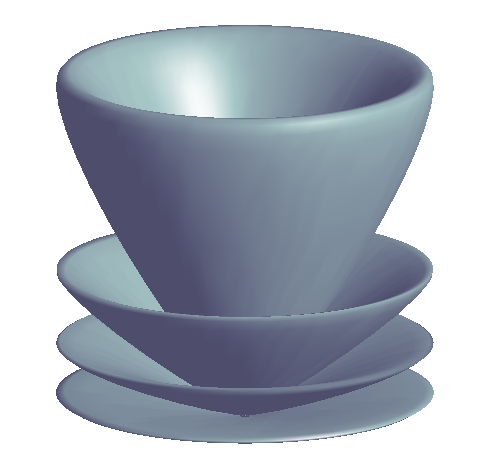
\includegraphics[width=\textwidth]{monopolepattern}
    \caption{Far-field radiation pattern of $4\lambda$ monopole~[Chetvorno, \texttt{CC0}].}
    \label{fig:radpat}
  \end{subfigure}
  \hspace{4em}
  \begin{subfigure}{.35\textwidth}
    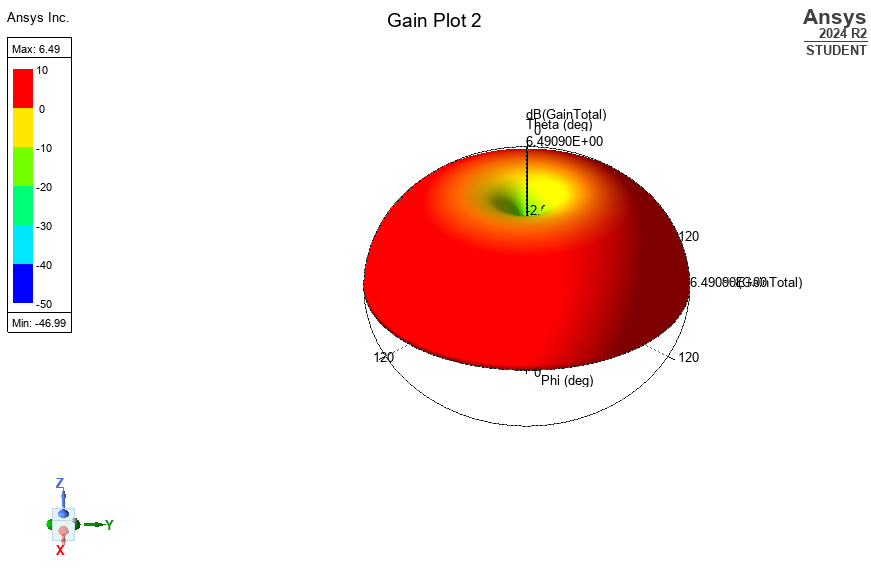
\includegraphics[width=\textwidth]{4lambda_monopole_antenna_gain}
    \caption{HFSS simulation results for $4\lambda=\qty{15}{\milli\meter}$ monopole antenna at \qty{8}{\giga\hertz}. $G=\qty{6.49}{\decibel}$.}
    \label{fig:hfss}
  \end{subfigure}
  \caption{$4\lambda$ monopole antenna analysis.}
\end{figure}
 
To estimate the gain of a $4\lambda$ antenna for an \qty{8}{\giga\hertz} uplink, a model in Ansys HFSS was used, which resulted in the 3D gain plot in Figure~\ref{fig:hfss}, for a maximum gain of \qty{6.49}{\decibel}.
Why it doesn't match Figure~\ref{fig:radpat}, I'm not sure, but it should still serve well as the telecommand antenna(s), since the margin is still quite high.

The uplink ${C/N}_\text{achieved}$ was calculated using the following expression, where square brackets indicate logarithmic quantities:
\begin{equation}\label{eq:uplinkachieved}
  [C/N]_\text{achieved}=[P_t] + [G_t] + [G_r] - [L_\text{path}] - [L_\text{point}] - [L_\text{atmosphere}] - [k] -[T]-[B]
\end{equation}
Whereas the downlink ${C/N}_\text{achieved}$ was calculated using a slightly different methodology, where the minimum certifiable $G/T$ figure is found by~\cite[I, p. 40]{commlinks}:
\begin{equation}\label{eq:minGT}
  \frac GT\ge \qty{40.7}{\decibel}+20\log{\frac f4}
\end{equation}
where $G/T$ is in \si{\decibel\per\kelvin}, and $f$ is in \si{\giga\hertz}.
Since that's the minimum figure of merit to be certified for a ground station, I took that as the figure of merit for Gatineau.
Then,
\begin{equation}\label{eq:downlinkachieved}
  [{C/N}]_\text{achieved}=[P_t]+[G_t]+\left[\frac GT\right]-[L_\text{path}]-[L_\text{point}]-[L_\text{atmosphere}]-[k]-[B]
\end{equation}
The ground station transmit power and the satellite noise temperature were both assumed based on representative data in the SME-SMAD.
The $G/T$ figure in equation~\ref{eq:minGT} is specifically for Telesat certification, but that should be applicable given the age of the Gatineau station and Telesat's presence in the area.
The \qty{10}{\decibel} atmosphere loss is mostly an expression of an allowable margin for atmospheric losses.
Further analysis would be required to get an accurate estimate of expected atmospheric losses.
Typically, they should be pretty low, since the signal really doesn't spend much time passing through the atmosphere at all.

\subsubsection{Power Subsystem}\label{sys:power}

Given SARGE's highly inclined orbit, there is in fact no eclipse time at all since the orbital plane is at about a right angle to the ecliptic plane.
The solar panels were sized according to Table~21-12 in the SME-SMAD for preliminary solar array sizing (Appendix~\ref{app:refs}, Figure~\ref{fig:2112}).
The process is laid out in Table~\ref{tab:powersub}.

\begin{table}
  \centering
  %
  \begin{tabular}{c|ll|rl|l}
    \toprule
    Step & Description & & Value & Unit & Notes\\
    \midrule
    \multirow{3}{7em}{Requirements and Constraints} & Power required & $P_\text{req}$ & 1061 &\si{\watt} & \\
    & Eclipse duration & $T_e$ & 0 & \si{\second} & \\
    & Design lifetime & $L$ & 5 & \si{yr} & \\
    \midrule
    \multirow{4}{7em}{Power to be produced} & Light duration & $T_d$ & 86170.5 & \si{\second} & $=P-T_e$\\
    & Path efficiency, eclipse & $X_e$ & 0.65 & & Unused\\
    & Path efficiency, day & $X_d$ & 0.85 & & Direct energy transfer\\
    & Required array power & $P_\text{sa}$ & 1,248 & \si{\watt} & $=P_\text{req}/X_d$\\
    \midrule
    \multirow{2}{7em}{Type of solar panel} & GaAs efficiency & $\eta$ & 18.5 & \si{\percent} & \\
    & Worst case power per cell & $P_0$ & 244.4 & \si{\watt\per\meter\squared} & $=\eta\cdot 1321$ SS\\
    \midrule
    \multirow{3}{7em}{BOL areal capacity} & Inherent degredation & $I_d$ & 0.72 & & Nominal\\
    & Worst case incident angle & $\theta$ & 10 & \si{\degree} & Appendix~\ref{app:orbplanes}\\
    & BOL performance & $P_\text{BOL}$ & 173.3 & \si{\watt\per\meter\squared} & $=P_0I_d\cos\theta$\\
    \midrule
    \multirow{3}{7em}{EOL production} & Degradation per year & $D$ & 2.75 & \si{\percent} & GaAs\\
    & Life degradation & $L_d$ & 0.87 & & $=(1-D)^L$\\
    & EOL performance & $P_\text{EOL}$ & 150.7 & \si{\watt\per\meter\squared} & $=L_dP_\text{BOL}$\\
    \midrule
    & Area needed & $A_\text{sa}$ & 8.28 & \si{\meter\squared} & $=P_\text{req}/P_\text{EOL}$\\
    & Mass & $M_\text{sa}$ & 22.36 & \si{\kilo\gram} & GaAs SJ, \qty{2.7}{\kilo\gram\per\meter\squared}\\
    & Price & & 1.063 & MM\$US & GaAs SJ, \qty{852}{\$\per\watt BOL}\\
    \bottomrule
  \end{tabular}
  \caption{Power subsystem solar array sizing.}
  \label{tab:powersub}
\end{table}

The only time a battery may be needed is during the ecliptic transfer orbit from launch to GEO.
The period $T$ of that orbit ($a=\qty{24364}{\kilo\meter}$, $T=2\pi\sqrt{a^3/\mu}$) is about \qty{10.5}{\hour}.
Being generous, we'll allow for 1.5 orbits (\qty{17.3}{\hour}) of primary battery power (i.e. one ``go-around'').
For this, we'll choose a \ce{LiSO2} battery system (chosen for the ``day-scale'' energy storage performance) with a specific energy density of \qty{350}{\watt\hour\per\kilo\gram}.
Assuming the payload is off during this transfer orbit, the power needed is \qty{711}{\watt}, and thus we need to store \qty{12.3}{\kilo\watt\hour} of energy, giving a battery mass of \qty{35}{\kilo\gram} (\qty{43}{\percent} of power subsystem mass).
The solar array takes up \qty{30}{\percent} of the power subsystem mass (with \qty{10}{\percent} margin), and the remaining \qty{22}{\kilo\gram} (\qty{27}{\percent}) is left for the harness with \qty{10}{\percent} margin.
Ideally, the spent primary battery would be ejected along with the kick motor to ease the fuel requirements for stationkeeping, but not for this current analysis.
The bus will be \qty{28}{\volt} to minimize current drawn and resistive losses, and since there's no eclipse, the bus will operate on direct energy transfer, without regulation.


\subsubsection{Thermal Control Subsystem}\label{sys:thermal}
To analyze the thermal situation of SARGE, the entire spacecraft body was assumed to be diffuse, gray, and isothermal.
Each principal axis was analyzed individually, for a total of 6 regions covering (1) the sides of sarge (along direction of travel); (2) the frontal (sun-facing) area of the solar panels only; (3) the frontal area of the spacecraft body only; (4) the bottom of the spacecraft (nadir pointing); (5) the entire back area of the solar panels and body; and (6) the top surface of the spacecraft.
The thickness of the solar panels was considered negligible.

The worst-case hot and cold calculations are shown in Table~\ref{tab:thermal}.

\begin{landscape}
  \begin{table}[h]
    \centering
    %\captionsetup
    \begin{tabularx}{1.00\linewidth}{ll|r|rrrrrr|l|X}
      \toprule
      WCH & & Total & Sides & F. Solar & F. Body & Bottom & Back & Top & Unit & Notes\\
      \midrule
      Material & & & 5ST & GaAs & 5ST & Z93 & Z93 & 2ST & & Material key follows table\\
      \midrule
      Solar Irradiance & $G_s$ & & 49.59 & 1421 & 1421 & 2.48 & 0 & 2.48 & \si{\watt\per\meter\squared} & WS, \ang{2} nadir error, \ang{0.1} rest error\\
      Solar absorption & $\alpha_s$ & & .07875 & .85575 & .07875 & .18375 & .18375 & .07875 & & \qty{5}{\percent} degradation EOL values\\
      IR emissivity & $\varepsilon_\text{IR}$ & & .741 & .57 & .741 & .874 & .874 & .627 & & GaAs ass. .6, and \qty{5}{\percent} EOL deg.\\
      Earth albedo & $\mathrm{a}$ & & & & & 35 &  & & \si{\percent} & +5\% albedo\\
      Earth IR flux & $\dot q_E$ & & 9 & 9 & 9 & 258 & 9 & 0 & \si{\watt\per\meter\squared} & High\\
      Generated power & $\dot Q_w$ & 844.33 & & & & & & & \si{\watt} & Justification following\\
      Area & $A_\text{sc}$ & 20.5 & 0.5 & 8.5 & 1 & 0.5 & 9.5 & 0.5 & \si{\meter\squared} & \\
      Earth ang. radius & $\rho$ & .15184 & & & & & & & \si{rad} & $=\sin^{-1}(R_E/r)$\\
      \midrule
      Sun IN & & 10,450 & 2 & 10,336 & 112 & 0 & 0 & 0 & \si{\watt} & $=G_s\alpha_s A_\text{sc}$\\
      Earth IR IN & & 0 & 0 & 0 & 0 & 0 & 0 & 0 & \si{\watt} & $=(\dot q_E\sin^2\rho)(1-\cos\rho)\varepsilon_\text{IR}/2$\\
      Albedo IN & & 0 & 0 & 0 & 0 & 0 & 0 & 0 & \si{\watt} & $=G_sA_\text{sc}\mathrm{a}\alpha_s(1-\cos\rho)\sin^2\rho/2$\\
      Total heat & $\dot Q_\text{out}$ & 11,295 & & & & & & & \si{\watt} & Including SC power gen\\
      \midrule
      Eff. emissive area & $\varepsilon_\text{IR}\cdot A_\text{sc}$ & 15.01 & 0.3705 & 4.845 & 0.741 & 0.437 & 8.303 & 0.3135 & \si{\meter\squared} & \\
      WCH Temperature & $T$  & 339.4 & & & & & & & \si{\kelvin} & $=\sqrt[4]{\dot{Q}_\text{out}/\sum{\varepsilon_\text{IR}A_\text{sc}}}=\qty{66.26}{\celsius}$\\
      \bottomrule\toprule
      WCC & & Total & Sides & F. Solar & F. Body & Bottom & Back & Top & Unit & Notes \\
      \midrule
      Solar Irradiance & $G_s$ & & 46.10 & 1321 & 1321 & 2.31 & 0 & 2.31 & \si{\watt\per\meter\squared} & SS, same errors\\
      Solar absorption & $\alpha_s$ & & .075 & .815 & .075 & .175 & .175 & .075 & & BOL\\
      IR emissivity & $\varepsilon_\text{IR}$ & & .78 & .65 & .78 & .92 & .92 & .66 & & BOL\\
      Earth albedo & $\mathrm{a}$ & & & &  & 25 & & & \si{\percent} & -5\% albedo\\
      Earth IR flux & $\dot q_E$ & & 7.54 & 7.54 & 7.54 & 216 & 7.54 & 0 & \si{\watt\per\meter\squared} & Low\\
      \midrule
      Sun IN & & 9,252 & 2 & 9,151 & 99 & 0 & 0 & 0 &\si{\watt} & Same calculations as WCH\\
      Total heat & $\dot Q_\text{out}$ & 10,097 & & & &  & & & \si{\watt} & Including SC power gen\\
      \midrule
      Eff. emissive area & $\varepsilon_\text{IR}\cdot A_\text{sc}$&16.23 & 0.39 & 5.525 & 0.78 & 0.46 & 8.74 & 0.33 & \si{\meter\squared}&\\
      WCC Temperature & $T$ & 323.7 & & & & & & & \si{\kelvin} & $=\qty{50.51}{\celsius}$\\
      \bottomrule
    \end{tabularx}
    \caption{Worst-case thermal calculations.}
    \label{tab:thermal}
  \end{table}
\end{landscape}
5ST and 2ST are 5~mil Silver-coated Teflon and 2~mil Silver-coated Teflon, respectively, and Z93 is the Z93~white paint.
Values for these materials were taken from Table~22-14 in SME-SMAD (Appendix~\ref{app:refs}, Figure~\ref{fig:2214}).
The first configuration for SARGE had the back surfaces covered in 2~mil Silver-coated Teflon, which resulted in a WCH temperature of \qty{81}{\celsius} and a WCC of \qty{64}{\celsius}.
Given the typical operating temperature ranges in Slideshow~10, Thermal, this range seemed high.
Changing the back surfaces to Z93~white paint resulted in a much milder steady-state situation.

The generated power of the spacecraft is lower than the total power in the power budget as I assumed that the \qty{100}{\watt} downlink transmitter power is emitted as signal (RF-waves) and that a third of the payload power (\qty{117}{\watt}) is similarly emitted as radar waves.
Since SARGE is quite far from the Earth, it makes sense that the reflected sunlight and Earth IR emissions are very low, essentially rounding errors. Their contributions are still included in the totals, but it is essentially negligible.

Galium Arsenside panels were assumed to be approximately \qty{100}{\percent} absorptive of solar energy~\cite{gaas}, with the \qty{18.5}{\percent} efficiency of electrical conversion taken into account.
The IR emissivity was estimated to be around 0.6, the lower end of Silicon cells.

\subsubsection{Guidance and Navigation Subsystem}\label{sys:nav}
Relevant perturbations and explanation (1)

orbit control strategy (maintenance, actuators/sensors) (2)

choice of autonomous or groun control with explanation/justification (2)

de-orbiting strategy and explanation (1)

\subsubsection{Propulsion Subsystem}\label{sys:prop}
Orbital transfer from injected orbit (calculations and justification for maneuver choice) (3)

Propellant mass calculations for maintenance and deo-orbiting (3) take from appendix and put here

Given the GTO... stationkeeping... disposal...

Can't use ion engine because of power requirements...\cite{next}

yeah
\subsubsection{Attitude Determination and Control Subsystem}\label{sys:adcs}
attitude control strategy and explanation/justification (2)

actuator selection and explanation/justification (1)

sensor selection and justification/explanation (2)

pointing requirements, maneuvers needed and explanation/justification (1)

\subsubsection{Structures}\label{sys:struct}
material selections and explanation/justification (2.5)

mechanism selection and explanation/justification (2.5)


\section{Launcher Selection Trade Study}\label{sec:launcher}
A selection of launch platforms still in use as of 2025 were considered, with the key parameters summarized in Table~\ref{tab:launchertrade}.
All launchers deliver their payload to GTO, with fairly minor differences in delivered transfer orbit, with the exception of the Ariane~62.

\begin{table}[h]
  \centering
  \captionsetup{width=.75\linewidth,font=small,labelfont=bf}
  \begin{tabular}{lc|cccc|ccr}
    \toprule
    Platform & Country & $i$ (\si{\degree}) & $h_p$ (\si{\kilo\meter}) & $h_a$ (\si{\kilo\meter}) & $\omega_p$ (\si{\degree}) & $M$ (\si{\kilo\gram}) & $D$ (\si{\meter}) & Cost \\
    \midrule
    SpaceX Falcon 9~\cite{spacex} & USA & \num{28.5} & \num{185} & \num{35788} & \num{0} & \num{5800}\textdagger & \num{3.7} & \num{69.75}~\cite{spacexprice} \\
    Ariane~62~\cite{ariane} & France & \num{6} & \num{250} & \num{35786} & \num{178} & \num{4500} & \num{5.4} & \num{88}\hspace{1.55em}\cite{arianeprice}\\
    Atlas V 401~\cite{atlasv} & USA & \num{27} & \num{185} & \num{35786} & \num{180} & \num{4750} & \num{4.0} & \num{109}\hspace{.6em} \cite{atlasvprice}\\
    Long March 3B~\cite{longmarch} & China & \num{28.5} & \num{200} & \num{35786} & \num{178} & \num{5100} & \num{4.0} & \num{70}\hspace{.9em}\cite{longmarchprice}\\
    \bottomrule
  \end{tabular}
  \caption{Selected launch platform comparison. \textdagger: includes payload adapter. Prices in millions USD, not adjusted for inflation.}
  \label{tab:launchertrade}
\end{table}

explain shared launch reasoning, or actually evaluate if shared launch is even possible given the huge propulsion requirements


\section{Schedule}
worth 2 marks :/

order of various design stages, can include chart (2)

\section{Cost}
worth 2 marks :/

major cost elements (launcher, payload, testing, insurance) (1)

reliable sources references (textbook, other missions, etc) (1)


\section{Conclusions}
summarize major values/parameters (3)

discuss future work (2)

Although further analysis is required to ensure that the current configuration can reject/retain enough heat, and the delta V budget is yet to be done, the current iteration of SARGE looks to be reasonable.
The mass distribution and total mass falls within the ranges typical of a GEO mission.
The total estimated power draw is somewhat lower than what is mentioned in the course slides.
The link budget has good margins, even after adding an assumed atmospheric loss.



\clearpage
\appendix

\printbibliography
\clearpage
\section{Orbital Perturbations and $\Delta V$}\label{app:orbpert}

SME-SMAD equations (9-46) and (9-47) on pg.~219 give approximate worse case $\Delta V$ relations per year~\cite{sme}:
\begin{align}
  {\Delta V}_\text{Moon} &= 102.67\cos\alpha\sin\alpha\hspace{2em}\text{(m/s per year)}\\
  {\Delta V}_\text{Sun} &= 40.17\cos\gamma\sin\gamma\hspace{2.7em}\text{(m/s per year)}
\end{align}
where $\alpha$ is the angle between the orbit plane and the Moon's orbit, and $\gamma$ is the angle between the orbit plane and the ecliptic.

\subsection{Stationkeeping}\label{app:stnkeep}
The angles estimated in Appendix~\ref{app:orbplanes} and illustrated in Figure~\ref{fig:moonorbit}, substituted into the preceding expressions, yield:
\begin{equation}
  {\Delta V}_\text{Moon} = 102.67\cos{\ang{92.42}}\sin{\ang{92.42}} = \qty{4.331}{\meter\per\second\per yr}
\end{equation}
\begin{equation}
  {\Delta V}_\text{Sun} = 40.17\cos{\ang{97.56}}\sin{\ang{92.42}} = \qty{5.239}{\meter\per\second\per yr}  
\end{equation}
And then, for the design lifetime of 5 years, the total $\Delta V$ for North-South stationkeeping is the product of the sum of the above:
\begin{equation}
  {\Delta V}_{NS} = ({\Delta V}_\text{Moon} + {\Delta V}_\text{Sun}) \times \qty{5}{yr} = \qty{47.85}{\meter\per\second}
\end{equation}
This is significantly less than the example value of about \qty{51.48}{\meter\per\second\per yr} given in the SME-SMAD for a GEO orbit with an inclination $i$ of \ang{0}~\cite{sme}.
This makes sense, since for a equatorial GEO orbit the Ecliptic and Lunar planes would be between \ang{23.44} and \ang{28.68}, whereas SARGE's highly inclined orbital plane is at nearly right angles to the Ecliptic and Lunar planes, somewhat balancing the perturbing forces of both.

The transverse (East-West) stationkeeping requirement is mentioned as about \qty{10}{\percent} of the North-South stationkeeping requirements~\cite{sme}, however I believe that the high inclination of SARGE will work against us in this scenario, as the oblateness of Earth around the equator will have a more pronounced effect for orbits that do not closely follow the equator.
As well, this oblateness likely has an effect on the North-South stationkeeping, since we're dealing with neither a polar nor equatorial orbit.
For this reason, I'm going to estimate the East-West stationkeeping to be equal to the North-South:
\begin{equation}
  {\Delta V}_{EW} = {\Delta V}_{NS} = \qty{47.85}{\meter\per\second}%pg 219
\end{equation}
This ought to roughly account for the stationkeeping requirements of the spacecraft at this stage of design. 

\subsection{Decommissioning}

The SME-SMAD recommends handling the special scarcity and properties of the GEO orbit (specifically its vulnerability to debris and junk) by raising spacecraft \qty{500}{\kilo\metre} above GEO at the end of their life.
The $\Delta V$ required for that is
\begin{equation}
  {\Delta V}_\text{disposal} = \qty{18}{\metre\per\second}
\end{equation}
from SME-SMAD page 233 for decommissioning a GEO satellite~\cite{sme}, and the propellant mass will be found at a later date after an in-depth $\Delta V$ analysis.

\subsection{Orbital Transfer}
The transfer from the SpaceX GTO orbit in Table~\ref{tab:launchertrade} will be a combined plane-change and elliptical-to-circular maneuver.
The $\Delta V$ required for such a change is~\cite{aero3240}:
\begin{equation}
  \Delta V=\sqrt{v_1^2+v_2^2-2v_1v_2\cos{\Delta i}}
\end{equation}
where $\Delta i=\ang{121}-\ang{28.5}=\ang{92.5}$, and $v_1,\,v_2$ are the orbital velocities of the transfer orbit and final orbit respectively.
The full calculation is scanned and attached in Appendix~\ref{app:orbcalcs}.
Hand calculations were chosen as a change of pace.
The final result is a $\Delta V$ of \qty{3.5253}{\kilo\meter\per\second}.


\section{Power and Configuration Implications}\label{app:powerandconf}
\subsection{Power Collection and Storage}\label{app:powercollection}
Given the estimated total average power presented in Table~\ref{tab:power}, \qty{1061}{\watt}, the required solar panel coverage can be estimated following the example in slide deck 7, ``Power'', where the following expression is provided on slide~17:
\begin{equation}
  {PD}_\text{out}={PD}_\text{in}\eta\cos\theta
\end{equation}
where ${PD}_\text{out/in}$ is the power density of out of and into the solar array in \si{\watt\per\meter\squared}, $\eta$ is the power conversion efficiency of the cells, and $\theta$ is the solar incident angle.
Taking the incident solar power as \qty{1366}{\watt\per\meter\squared}, and the achieved efficiency of GaAs cells provided in slide~18 of \qty{18.5}{\percent}, with a worst-case incident angle of about \ang{10} (since the angle of the orbital plane to the ecliptic is \ang{97.56}, found in Appendix~\ref{app:orbplanes}), then
\begin{equation}
  {PD}_\text{out}=\qty{1366}{\watt\per\meter\squared}\cdot\qty{18.5}{\percent}\cdot\cos(\ang{10})= \qty{248.87}{\watt\per\meter\squared}
\end{equation}
Then, dividing the total average power required by the spacecraft (and noting that the spacecraft spends no time in eclipse), the minimum required illuminated area of the solar array is
\begin{equation}
  A_\text{solar,min} = \frac{P_\text{total}}{PD_\text{out}} = \qty{4.26}{\square\meter}
\end{equation}
Since the spacecraft is orbiting in a plane nearly perpendicular to the ecliptic plane, a 1~DoF mechanism for the pointing of the solar array with an angular envelope of $\pm\ang{10}$ should be sufficient to ensure optimal solar collection.
This fact and the lack of eclipse time is well conveyed by Figure~\ref{fig:eclipse} below, showing no part of the orbital track lying in eclipse.

\begin{figure}[h]
  \centering
  \captionsetup{width=.75\linewidth,font=small,labelfont=bf}
  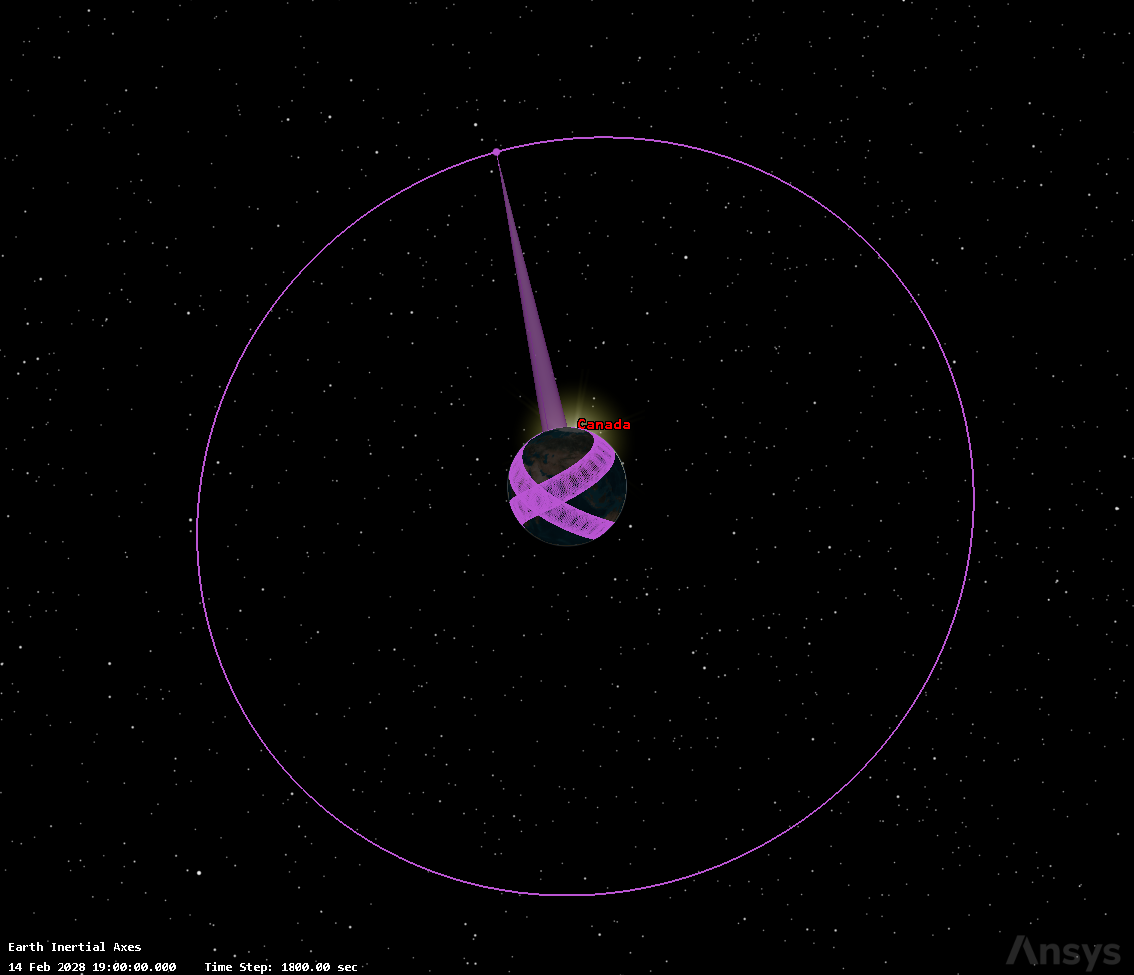
\includegraphics[width=8cm]{zeroeclipse}
  \caption{Demonstration of zero eclipse time via STK 3D view. The sun is visible just over the horizon.}
  \label{fig:eclipse}
\end{figure}

\subsection{Configuration Choices}
In order to accomodate the necessary surface area of the solar panels in a compact way with margins to account for structural frames that would block cells of the solar array, and to pre-emptively take into account the packing of the spacecraft into a launch platform, a quick sketch (Figure~\ref{fig:solarsketch}) showed that the structure should follow roughly a form factor of $\SI{1}{\meter}\times\SI{1}{\meter}\times\SI{0.5}{\meter}$.
This allows the compact packing of nominally \SI{6}{\square\meter} of solar panels, which well exceeds the required \SI{4.26}{\square\meter}.
In later analysis, it will be shown how much of a margin we have to block that area with support structures when EOL conditions and degradation is taken into account.

Table~21-5 in the SME-SMAD notes that travelling wave tube amplifiers (TWTA)s are about 50-60\% efficient for X-band and weigh about \qty{2.5}{\kilo\gram} including power converter~\cite[p. 637]{sme}.
Table~16-16 in the SME-SMAD notes that parabolic reflectors weigh between 10-30~kg~\cite[p. 484]{sme}.

\clearpage
\section{Fun!}
This section is named ``Fun!'' unironically -- these were fun.

\subsection{Fun Annulus Geometry}\label{app:annulus}
To approximate the arc angle subtended by the \ang{10} elevation $\delta$ access requirement, I created a quick sketch shown in Figure~\ref{fig:annulus} to wrap my head around the geometry.
I then used the formula for worst-case distance $d$ from slide deck 6 to find the corresponding half angle $\gamma$:
\begin{equation}
  d=R_\text{Earth}\left(
    \sqrt{\left(\frac{r}{R_\text{Earth}}\right)^2-\cos^2\delta}
    -\sin\delta
  \right)
\end{equation}
From my sketch,
\begin{equation}
  \gamma = \sin^{-1}\left(\frac{d\sin(\ang{90}+\delta)}{r}\right)
\end{equation}
And thus the access ratio is the ratio between the access arc and the total arc (circumference):
\begin{equation}
  \text{Access Ratio} = \frac{2\gamma r}{2\pi r} = \qty{39.69}{\percent}
\end{equation}

\begin{figure}[h]
  \centering
  \captionsetup{width=.75\linewidth,font=small,labelfont=bf}
  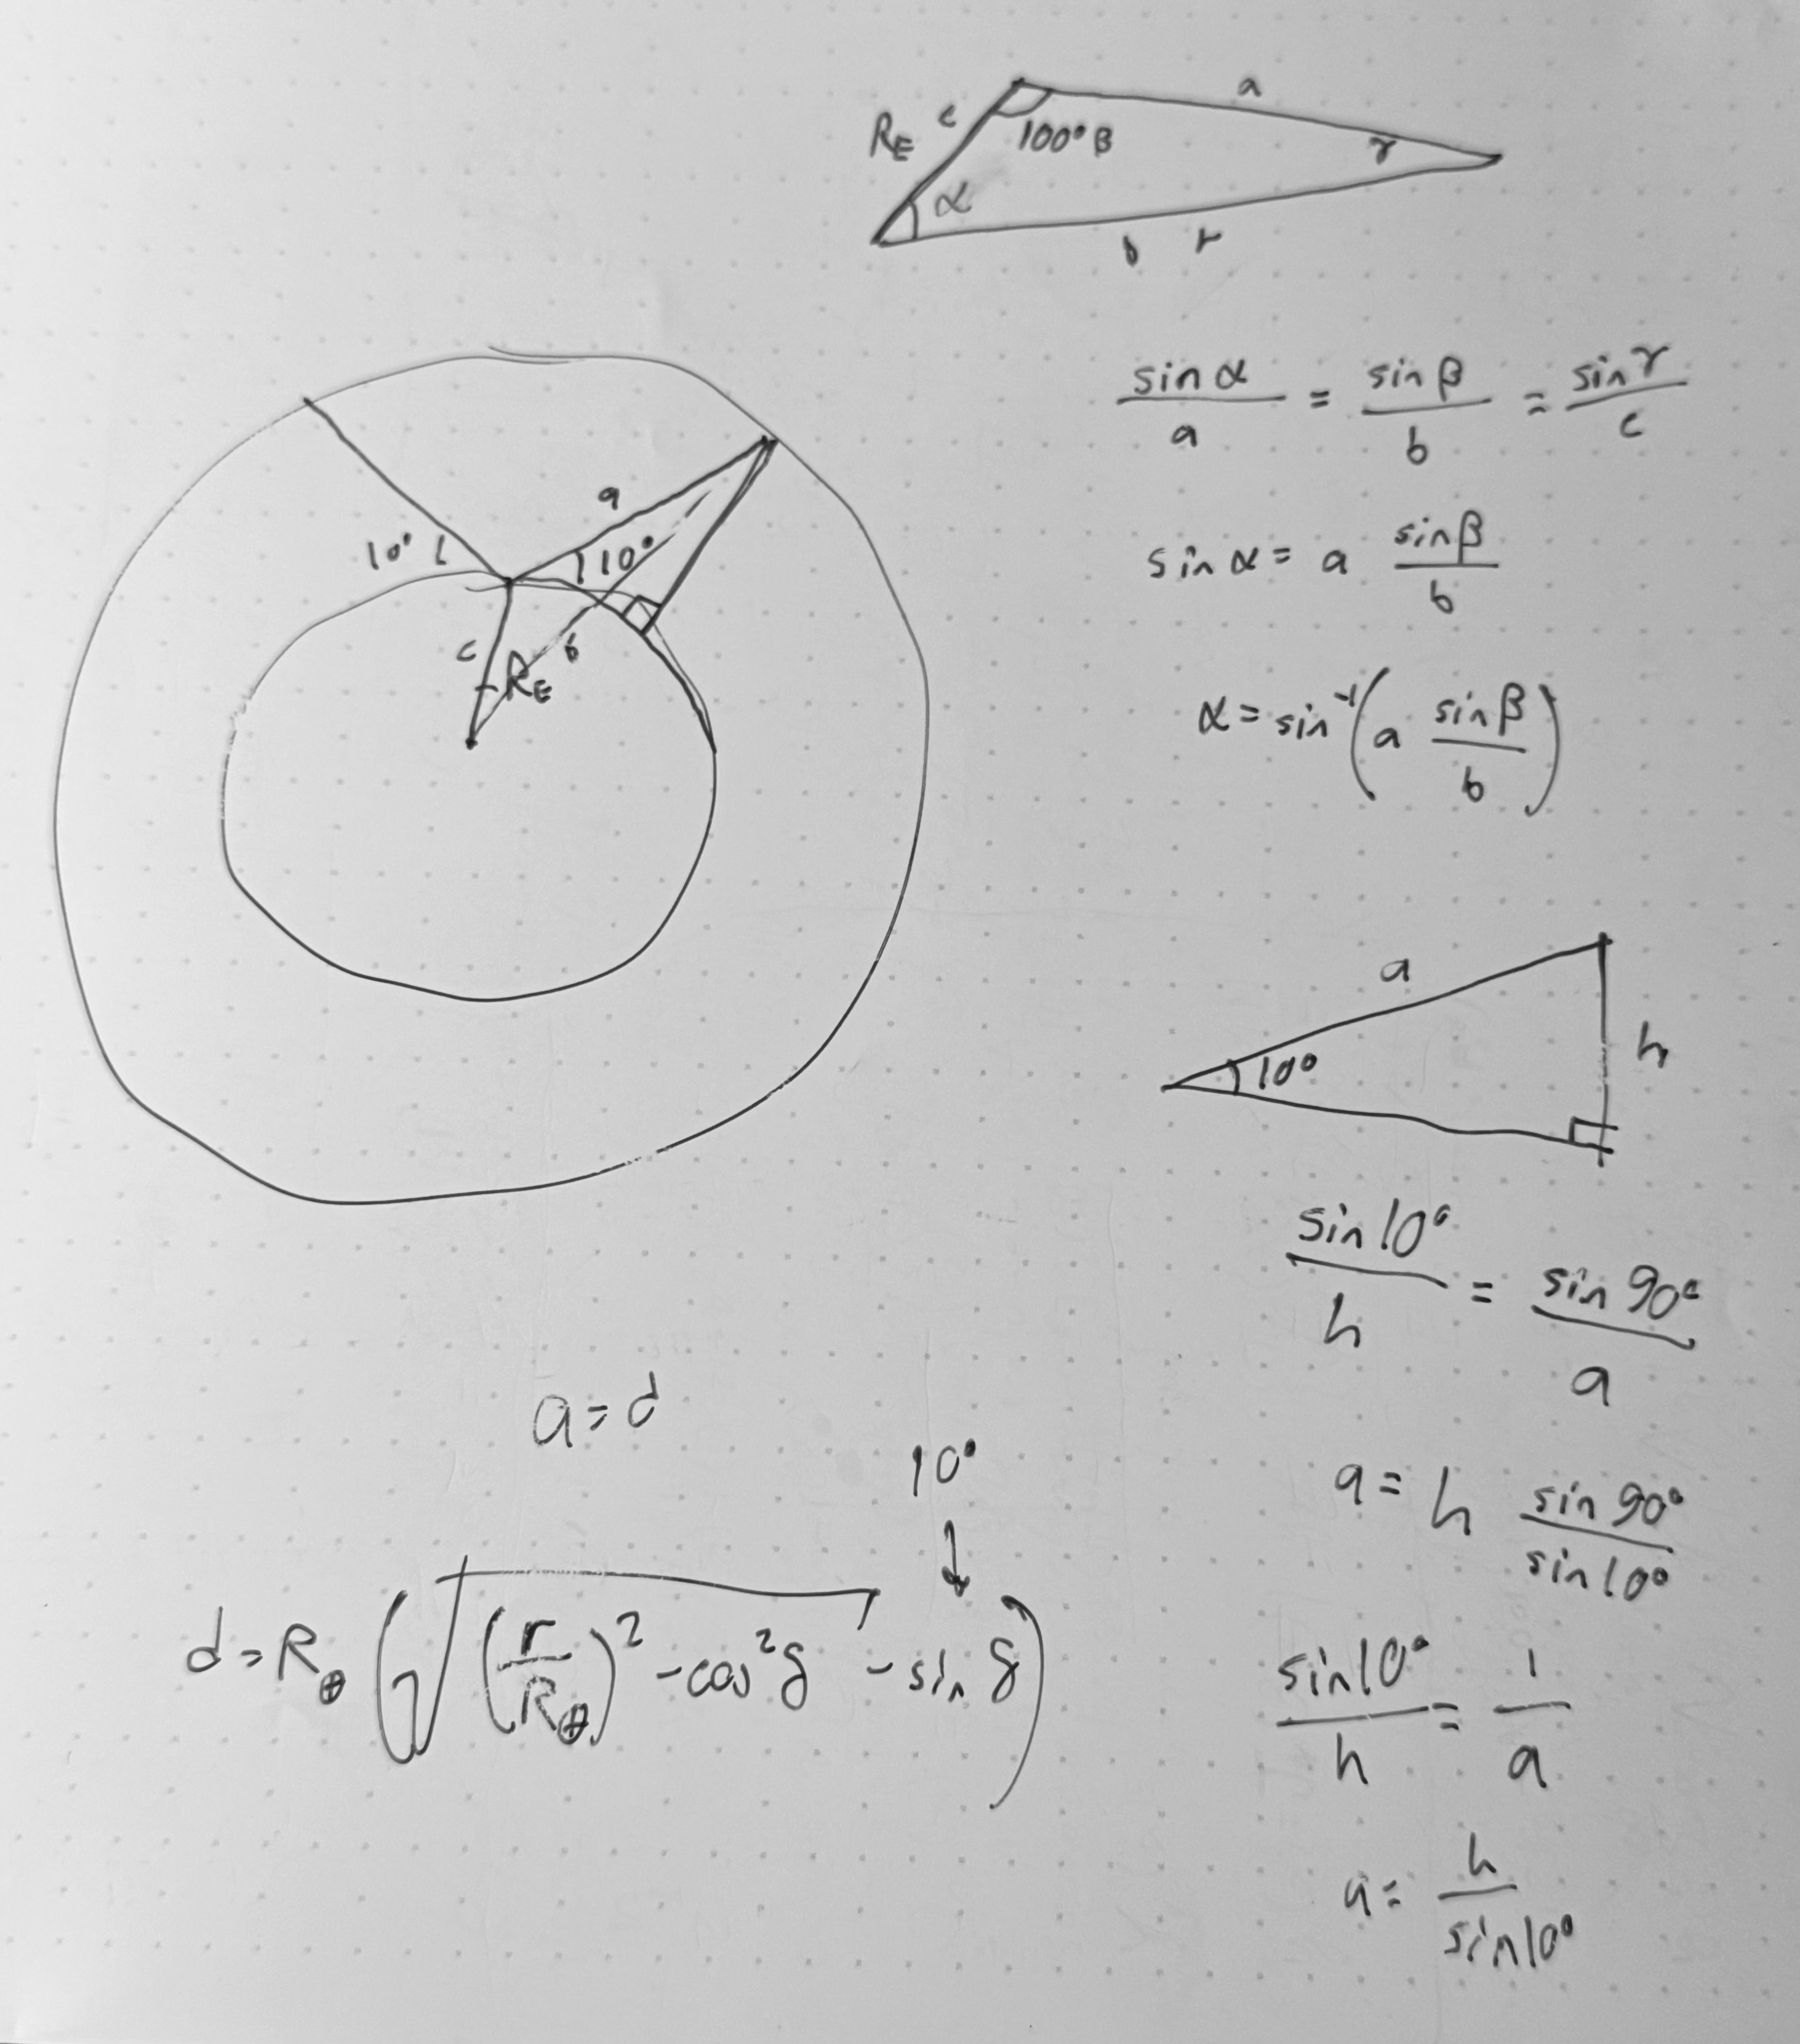
\includegraphics[width=10cm]{annulus}
  \caption{Figuring out the geometry to find the half-angle from the center of the Earth given the radius and elevation [Own work].}
  \label{fig:annulus}
\end{figure}

This makes a lot of sense -- SARGE is far away, the elevation angle of \ang{10} is pretty generous, and the groundtrack passes fairly close to Gatineau station (on a global scale, at least).

\subsection{Fun Orbital Plane Geometry}\label{app:orbplanes}

To find $\alpha$ and $\gamma$ for the orbital perturbation estimations in Appendix~\ref{app:orbpert}, I estimated the angles between SARGE's orbital plane and the Sun and the Moon using the Ecliptic plane and Lunar orbit inclination values found in a figure (with no listed author) from Wikipedia.

\begin{figure}[hb]
  \centering
  \captionsetup{width=.75\linewidth,font={small},labelfont={bf}}
  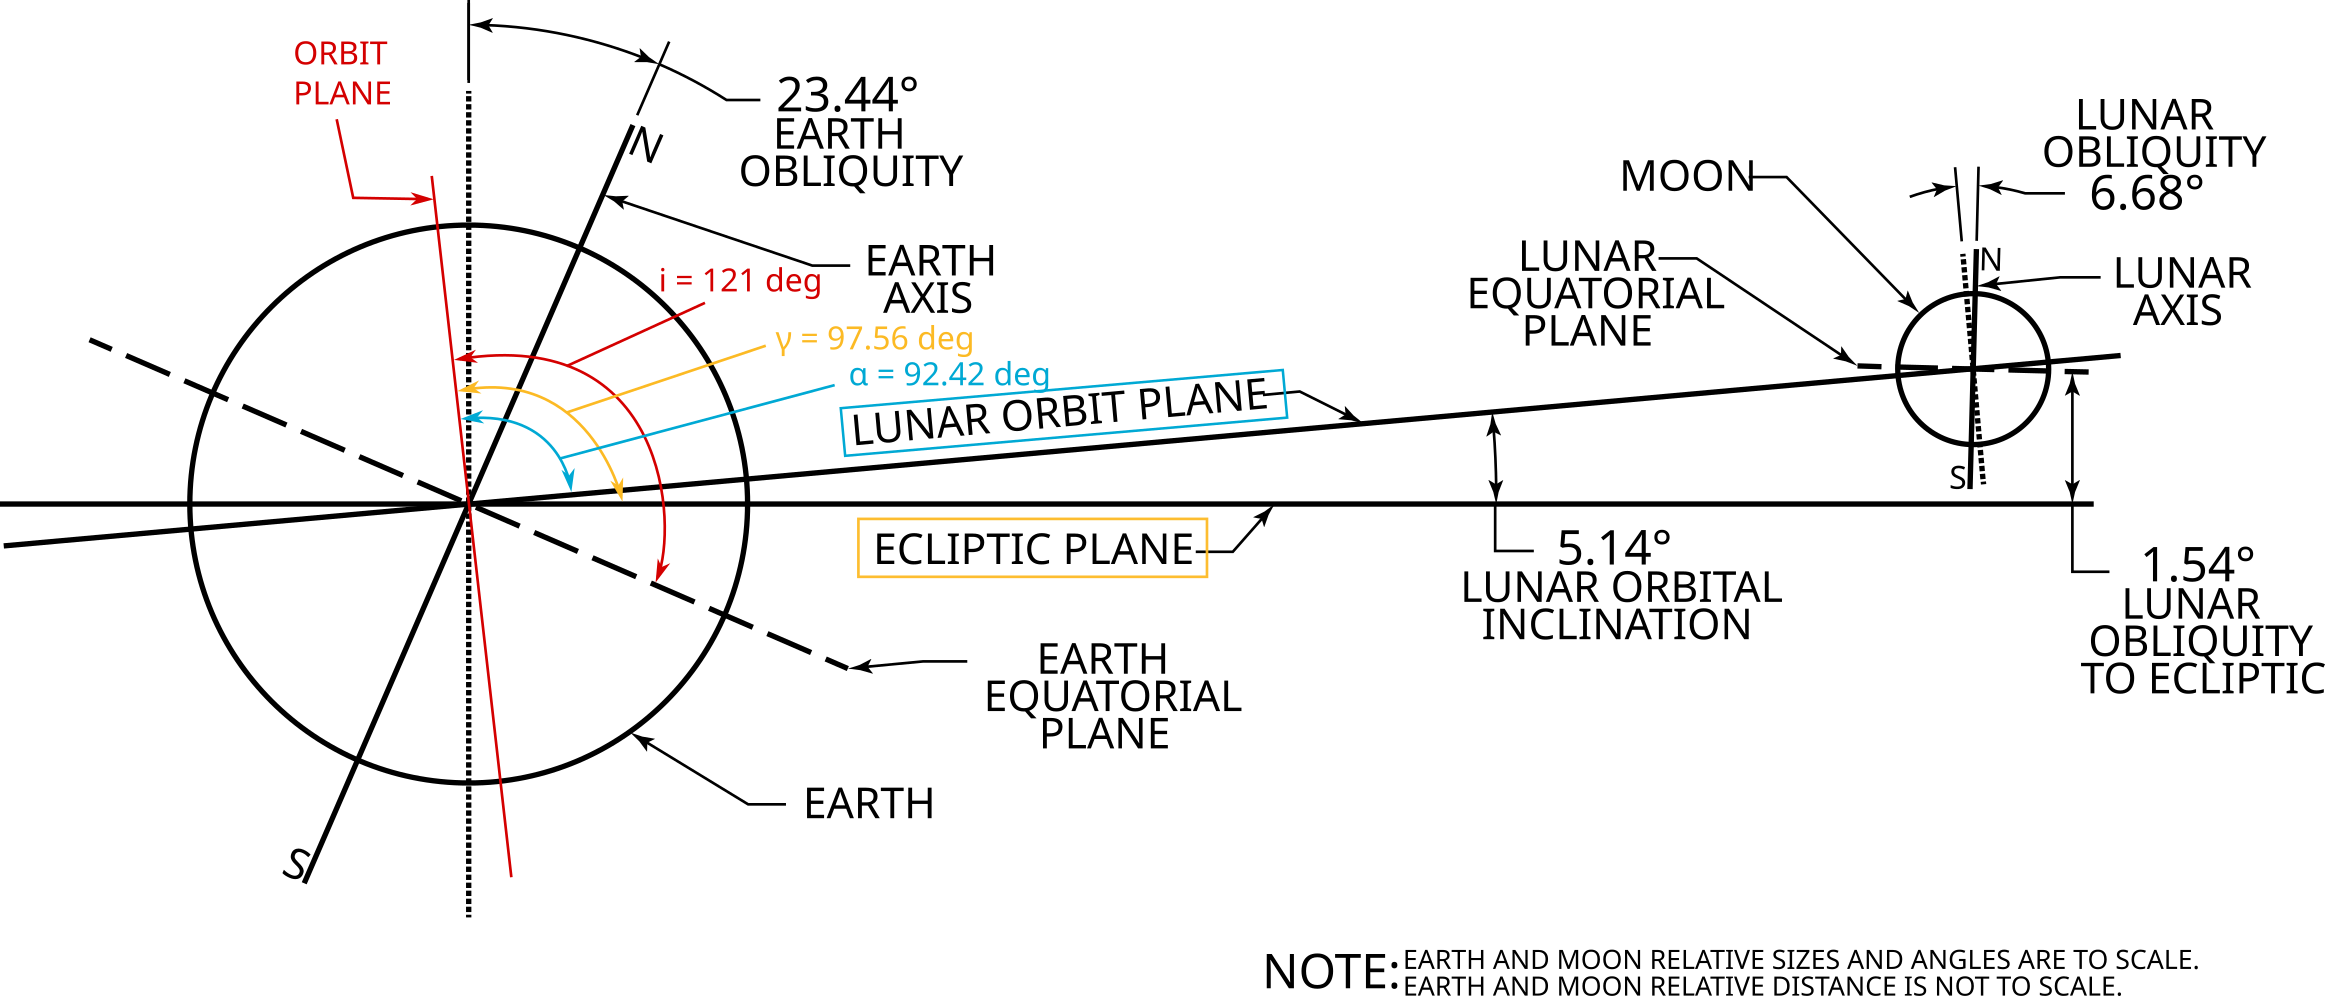
\includegraphics[width=15cm]{Annotated_Moon_Orbit}
  \caption{Angles between the orbit plane of SARGE and the Lunar orbit plane ($\alpha$) and the Ecliptic plane ($\gamma$). [Author unknown, \texttt{CC0}, annotations (in colour) added]}
  \label{fig:moonorbit}
\end{figure}

From Figure~\ref{fig:moonorbit}, we can estimate that the angle between SARGE's orbit plane and the Ecliptic plane ($\gamma$) to be \ang{97.56}, and between SARGE's orbit plane and the Lunar orbit plane ($\alpha$) as \ang{92.42}.

\section{Link Budget}\label{app:linkbudget}
\subsection{Down}
The initial step of developing the link budget is to determine how much payload data we need to download.
The area of Canada proper, shown in red in Figure~\ref{fig:groundtrack}, is about \qty{8.342e6}{\kilo\meter\squared}.
From the mission requirements, we need to image that entire area (at least) once every \qty{14}{\day}.
Assuming that the payload is capable of steering its beam in order to cover swaths of \qty{100}{\kilo\meter} width, and considering an image to be $\qty{100}{\kilo\meter}\times\qty{100}{\kilo\meter}$, with a linear resolution of \qty{5}{\meter} such that each pixel is $\qty{25}{\meter\squared}$ and contains \qty{16}{\bit} of data, we estimate the amount of data required to image all of Canada using the following:
\begin{equation}
  \text{Image Pixels} = \frac{\text{Image Area}}{(\text{Linear Resolution})^2}=\qty{4.0e8}{pixels}
\end{equation}
Then, the size of each image:
\begin{equation}
  \text{Image Size} = \text{Pixel Size}\times\text{Image Pixels} = \qty{800}{\mega\byte}
\end{equation}
Then, the images required to cover Canada, with a 4\% swath overlap accomodation:
\begin{equation}
  \text{Images per Canada} = \frac{A_\text{Canada}}{\text{Image Area}}\times 1.04 \approx \qty{868}{images}
\end{equation}
And thus, the amount of data required to image Canada once:
\begin{equation}
  \text{Canada Size} = \text{Images per Canada} \times \text{Image Size} = \qty{694.05}{\giga\byte}
\end{equation}
Over \qty{14}{\day}, the average payload data rate is then:
\begin{equation}
  R_\text{payload,avg} = \frac{\text{Canada Size}}{\qty{14}{\day}}=\qty{573.78}{\kilo\byte\per\second}
\end{equation}

This does not include the housekeeping data specified in the mission requirements and summarized in Table~\ref{tab:housekeepingdata} below.
\begin{table}[hb]
  \centering
  \captionsetup{width=.75\linewidth,font=small,labelfont=bf}
  \begin{tabular}{c|rl}
    \toprule
    Data & Quantity & Unit\\
    \midrule
    Error Detection & \num{3} & \si{\bit\per\byte}\\
    Latitude & \num{32} & \si{\bit\per image}\\
    Longitude & \num{32} & \si{\bit\per image}\\
    Altitude & \num{32} & \si{\bit\per image}\\
    Time & \num{64} & \si{\bit\per image}\\
    Synchronization & \num{24} & \si{\bit\per image}\\
    Health Data Rate & \num{26.66}\dots & \si{\bit\per\second}\\
    \bottomrule
  \end{tabular}
  \caption{Summary of required housekeeping data per mission requirements.}
  \label{tab:housekeepingdata}
\end{table}

\noindent The total housekeeping data per image can then be found via
\begin{multline}
  \text{Housekeeping per Image} = \text{Image Size}\times\text{Error Detection}+\text{Latitude}+\text{Longitude}\\+\text{Altitude}+\text{Time}+\text{Synchronization} = \qty{300}{\mega\byte\per image}
\end{multline}
The total housekeeping data per Canada:
\begin{equation}
  \text{Housekeeping Size} = \text{Housekeeping per Image} \times \text{Images per Canada} = \qty{260.27}{\giga\byte}
\end{equation}
And the average housekeeping data rate:
\begin{equation}
  R_\text{housekeeping,avg} = \frac{\text{Housekeeping Size}}{\qty{14}{\day}}+\text{Health Data Rate}=\qty{215.17}{\kilo\byte\per\second}
\end{equation}
To penultimately culminate in the \textit{average} downlink data rate:
\begin{equation}\label{eq:avgdownlinkdatarate}
  R_\text{DL,avg}=R_\text{payload,avg}+R_\text{housekeeping,avg}=\qty{788.95}{\kilo\byte\per\second}
\end{equation}
And as found in Appendix~\ref{app:annulus}, the proportion of time SARGE is within \ang{10} elevation of Gatineau is \qty{39.69}{\percent}, and thus the total access time is:
\begin{equation}\label{eq:totalaccess}
  T_\text{access} = P\times\qty{39.69}{\percent}\approx\qty{9.5}{\hour\per\day}
\end{equation}
From the guidance given in class, approximately \qty{20}{\percent} of access window should be allocated to uplink, thus the downlink window is \qty{80}{\percent} of $T_\text{access}$, and the actual downlink rate can be found:
\begin{equation}
  R_\text{DL} = \frac{R_\text{DL,avg}}{\frac{\qty{80}{\percent}\times T_\text{access}}{P}}=\qty{2.485}{\mega\byte\per\second}
\end{equation}
So the downlink rate required is about \qty{2.485}{\mega\byte\per\second}, which transmits for about \qty{7.6}{\hour} every sidereal day.
The bandwidth for QPSK (our downlink encoding scheme) is:
\begin{equation}
  B=0.6R=\qty{11.928}{\mega\hertz}
  \label{eq:downlinkbw}
\end{equation}

Then, as noted in Section~\ref{sec:configuration}, the communications satellite on SARGE is a parabolic antenna with a diameter $D_t$ of \qty{0.5}{\meter}.
Assuming a transmission efficiency $\eta_t$ of \qty{50}{\percent}, and noting that the wavelength $\lambda$ of the downlink center frequency of \qty{7.275}{\giga\hertz} is \qty{4.12}{\milli\meter}, the predicted gain is
\begin{equation}\label{eq:100}
  G_t=\eta_t\left(\frac{\pi D_t}{\lambda}\right)^2=\num{726}
\end{equation}

The path loss for the downlink direction is:
\begin{equation}\label{eq:101}
  L_\text{path}=\left(\frac{4\pi d}{\lambda}\right)^2\approx\num{6.53e-21}
\end{equation}
And the pointing accuracy loss can be estimated by finding the $\theta_{\qty{3}{\decibel}}$ angle via the relationship in slide deck 6:
\begin{equation}
  \theta_{\qty{3}{\decibel}}\approx\ang{70}\frac{\lambda}{D}=\ang{5.77}
\end{equation}
and then, assuming a pointing error $\epsilon$ of \ang{1} for the spacecraft:
\begin{equation}\label{eq:302}
  [L_\text{point}]=12\left(\frac{\epsilon}{\theta_{\qty{3}{\decibel}}}\right)^2=\qty{0.361}{\decibel}
\end{equation}

And finally, to find the required carrier to noise ratio, with a minimum bit error rate ${BER}$ of \num{10e-5} for the downlink, as suggested in slide deck 6:
\begin{equation}\label{eq:102}
  {C/N}_\text{required}=\frac RB\ln\left(\frac{1}{2{BER}}\right)=\qty{14.20}{\decibel}
\end{equation}

Whew.
\subsection{Up}
The uplink analysis is much the same as the downlink analysis presented just previously, except we just assume a transmission rate of \qty{2.5}{\kilo\bit\per\second}, and we're using BFSK as recommended in slide deck 6.
As well, for lack of better information and based on the ballparks present in the SME-SMAD, we assume a transmitter power at the basestation of \qty{200}{\watt}.
From Natural Resources Canada, the diameter of the Gatineau satellite dish is \qty{13}{\meter}, and we'll assume a pointing accuracy $\epsilon$ of \ang{0.25} and still a transmit efficiency $\eta_t$ of \qty{50}{\percent}.
Then the transmitter gain is:
\begin{equation}\label{eq:200}
  G_t=\eta_t\left(\frac{\pi D_t}{\lambda}\right)^2=\num{594e3}
\end{equation}
And the path loss is slightly different because the uplink center frequency is \qty{8.00}{\giga\hertz} with a corresponding wavelength $\lambda$ of \qty{3.75}{\milli\meter}:
\begin{equation}\label{eq:203}
  L_\text{path}=\left(\frac{4\pi d}{\lambda}\right)^2\approx\num{5.40e-21}
\end{equation}
And the $\theta_{\qty{3}{\decibel}}$:
\begin{equation}
  \theta_{\qty{3}{\decibel}}\approx\ang{70}\frac{\lambda}{D}=\ang{0.20}
\end{equation}
With a pointing loss of:
\begin{equation}\label{eq:303}
  [L_\text{point}]=12\left(\frac{\epsilon}{\theta_{\qty{3}{\decibel}}}\right)^2=\qty{18.42}{\decibel}
\end{equation}
A bandwidth of (according to slide deck 6):
\begin{align}
  B =2R(1+\beta)&=\qty{5016}{\hertz}\\\label{eq:201}
  \beta =\Delta f/f_{mod}&=\num{0.003125}\\
  \Delta f&=\qty{25}{\mega\hertz}\qquad(\text{Half of max channel BW})
\end{align}

And finally, the minimum carrier to noise is calculated in the same was as Eq.~\ref{eq:102}, but with a ${BER}$ of \num{10e-7} for telecommand, also as mentioned in slide deck 6:
\begin{equation}\label{eq:202}
  {C/N}_\text{required}=\frac RB\ln\left(\frac{1}{2{BER}}\right)=\qty{8.16}{\decibel}
\end{equation}
\clearpage
\section{Referenced Tables and Figures}\label{app:refs}
\begin{figure}[h]
  \centering
  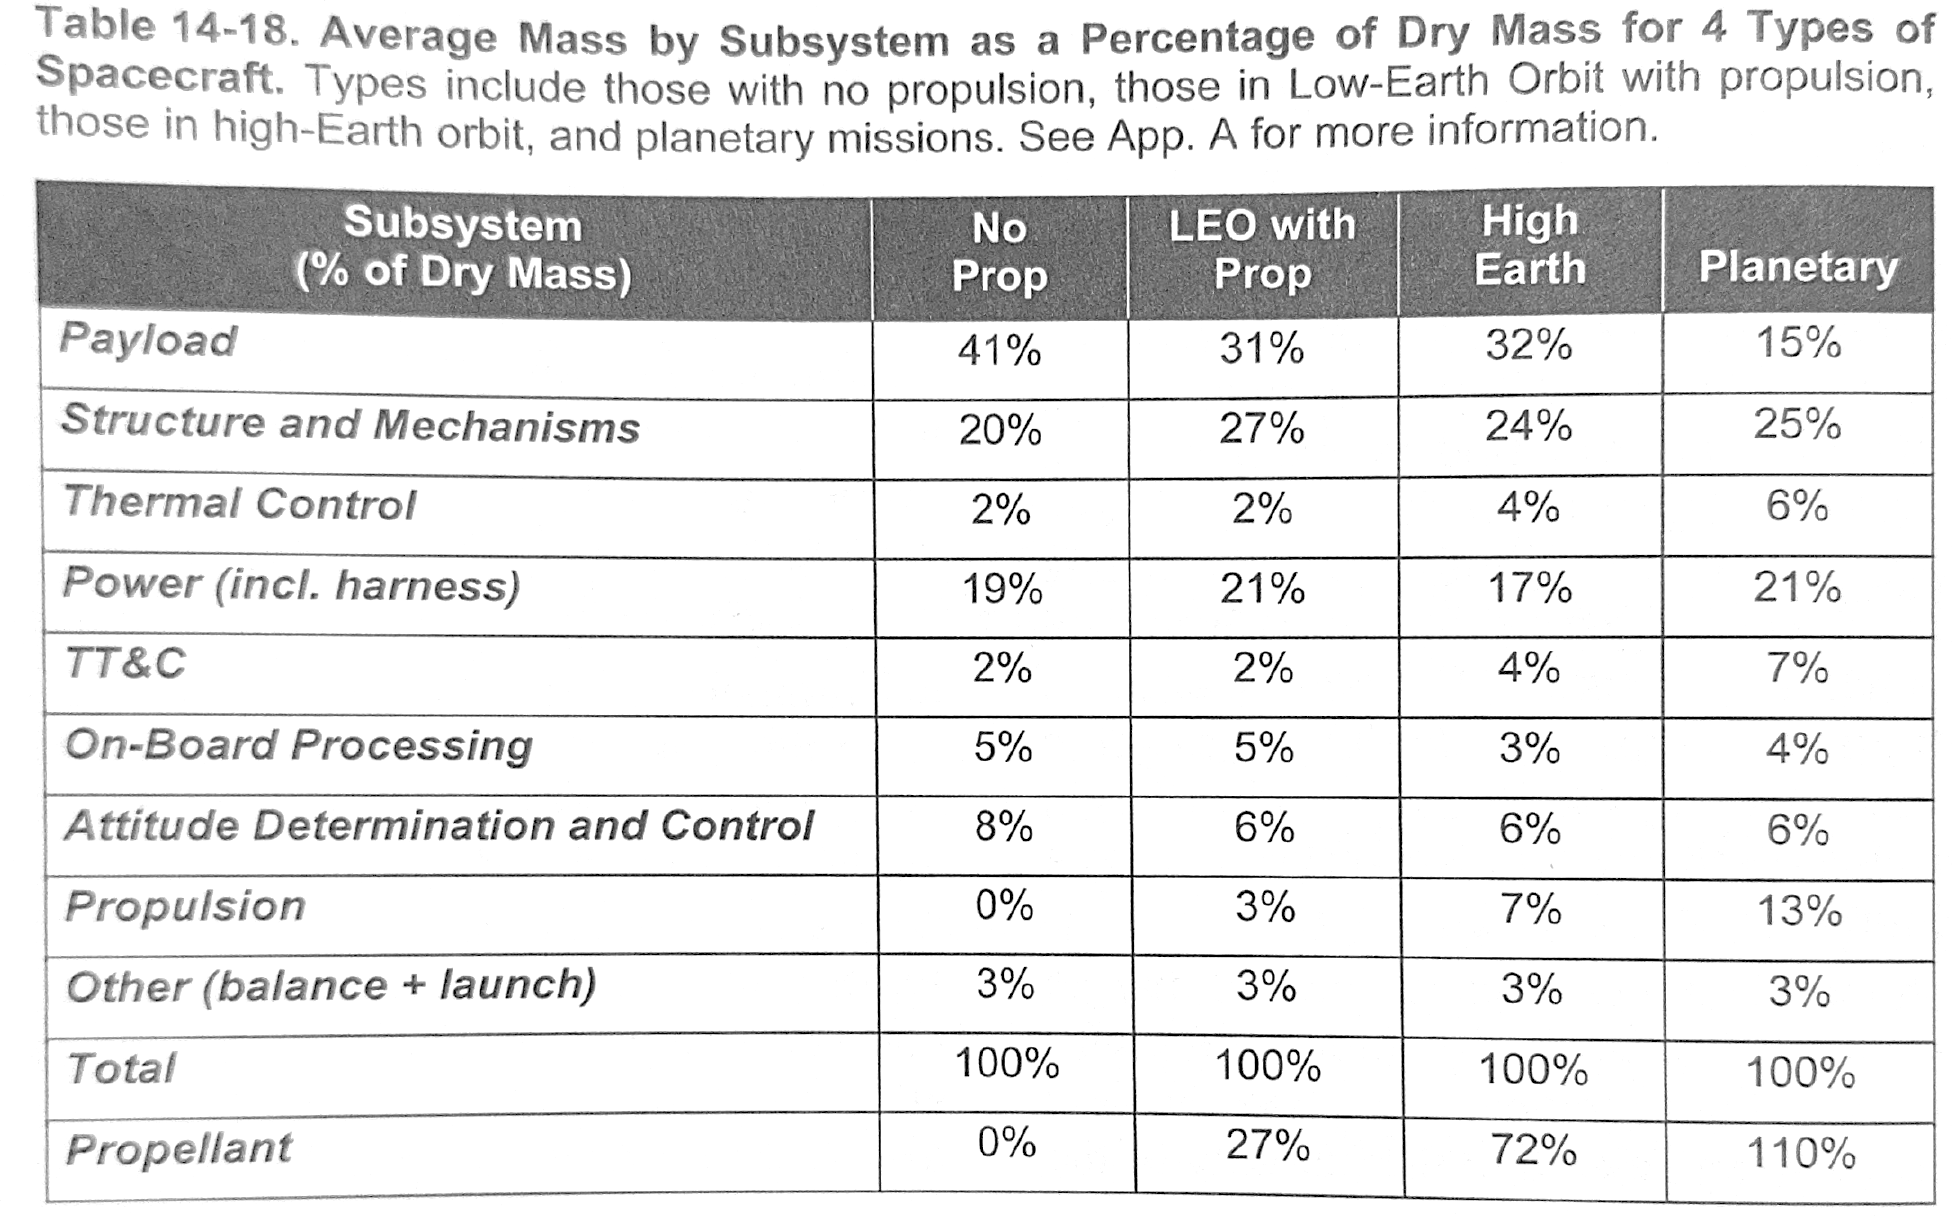
\includegraphics[width=.8\textwidth]{1418}
  \caption{Table 14-18 in SME-SMAD~\cite[p. 422]{sme}.}
  \label{fig:1418}
\end{figure}
\begin{figure}[h]
  \centering
  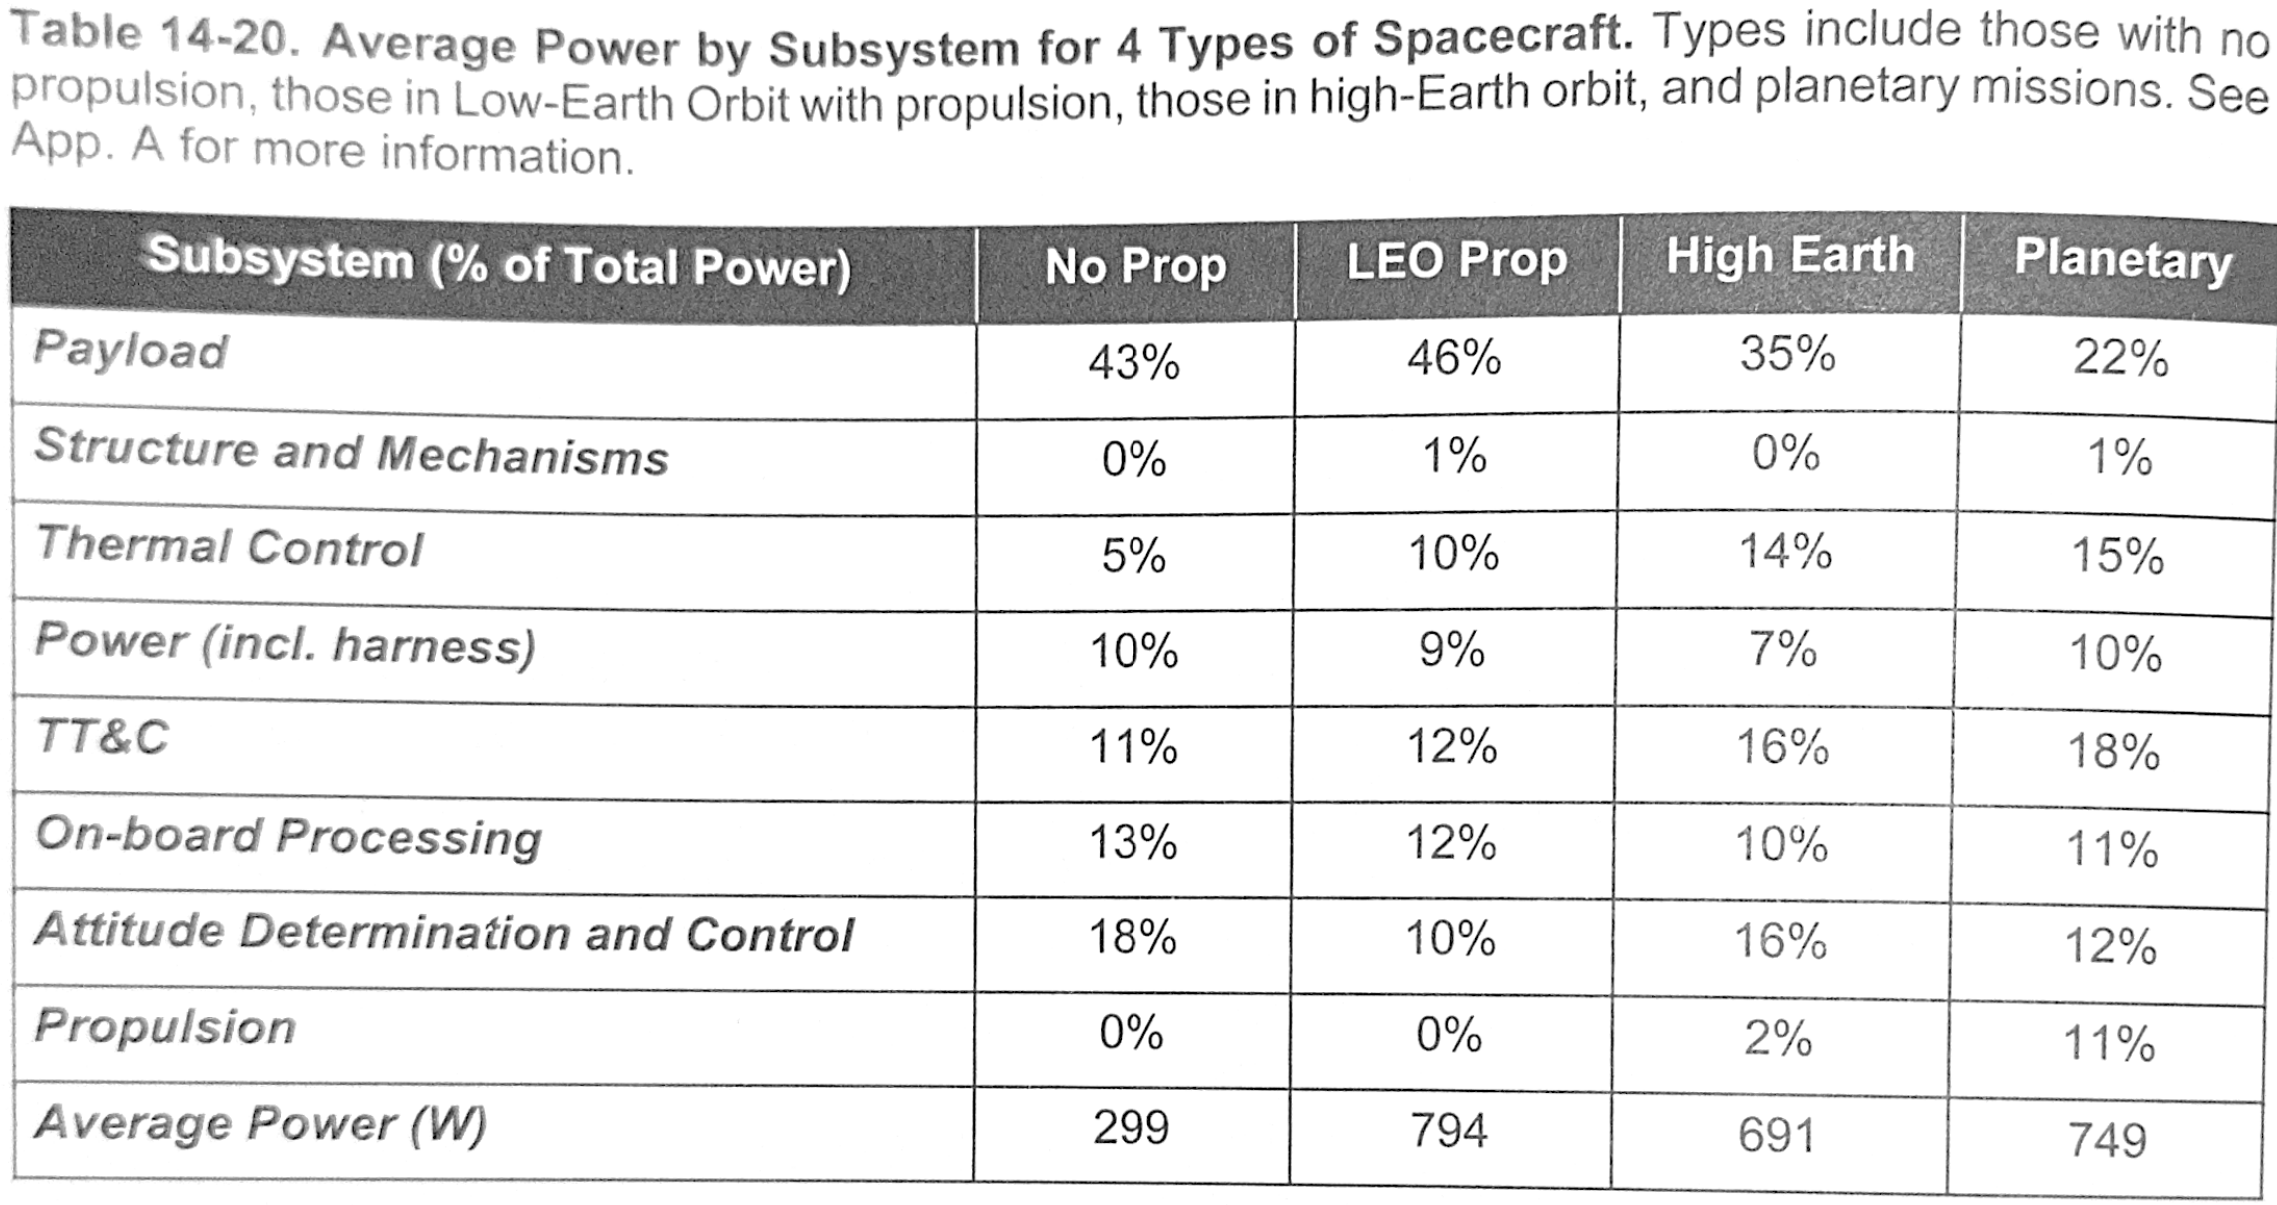
\includegraphics[width=.8\textwidth]{1420}
  \caption{Table 14-20 in SME-SMAD~\cite[p. 424]{sme}.}
  \label{fig:1420}
\end{figure}
\begin{figure}[h]
  \centering
  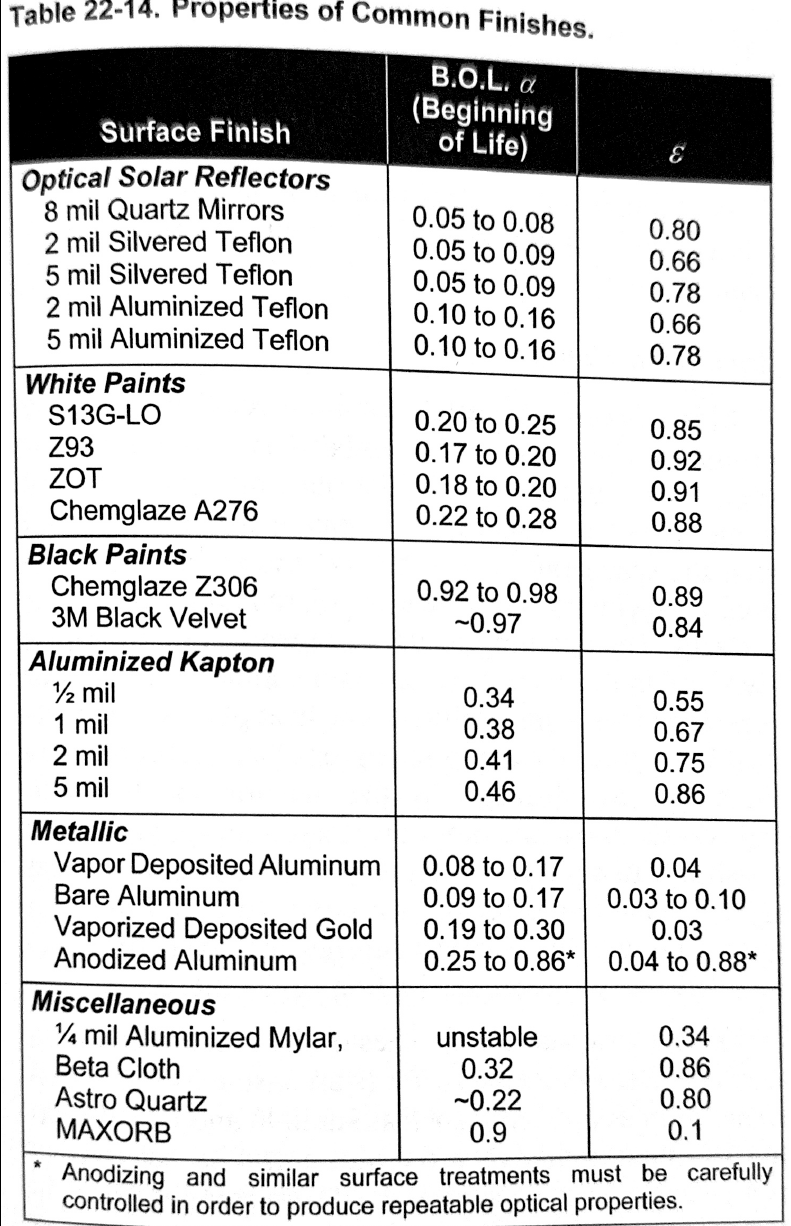
\includegraphics[width=.4\textwidth]{2214}
  \caption{Table 22-14 in SME-SMAD~\cite[p. 695]{sme}.}
  \label{fig:2214}
\end{figure}
\begin{figure}[h]
  \centering
  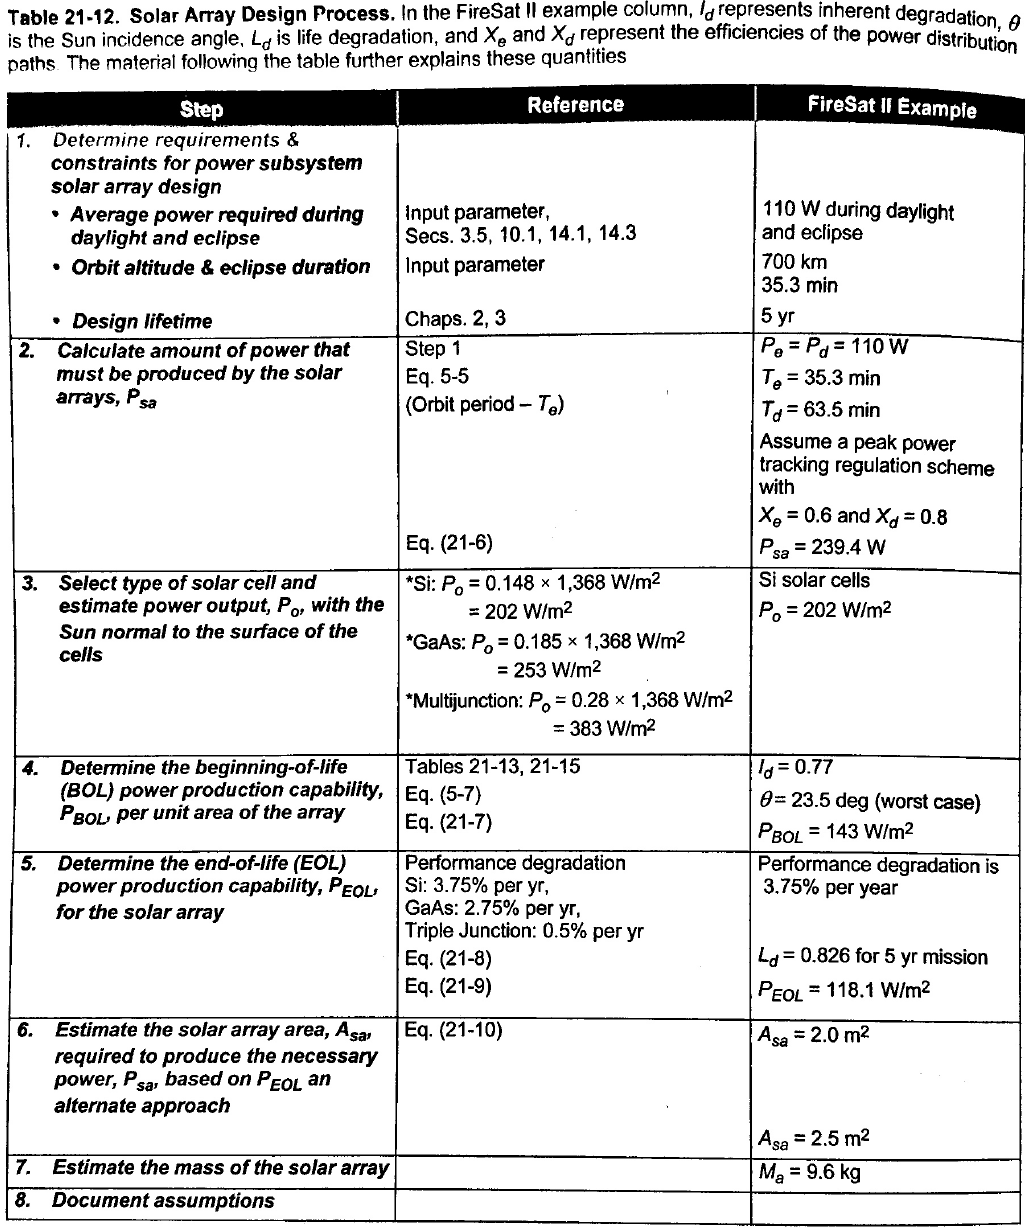
\includegraphics[width=.8\textwidth]{2112}
  \caption{Table 21-12 in SME-SMAD~\cite[p. 644]{sme}.}
  \label{fig:2112}
\end{figure}


\clearpage
\section{Orbital Transfer Calculations}\label{app:orbcalcs}
figure


\vfill
\section{Preliminary Drawings}\label{app:julia}


\end{document}
